\graphicspath{{3greece/asy/},{3greece/pics/}}

\section{Ancient Greek Mathematics}

\subsection{Overview of Ancient Greek Civilization \& Early Philosophy}

Greek civilization dates from around 800\BC, centered between the Adriatic sea to the west and the Aegean to the east. The ancient Greeks had a decentralized political culture consisting of mostly independent city-states connected by trade. By 500\BC{}, much of modern Greece, the Aegean islands, and southern Italy were part of a decentralized cultural empire. Accomplished sea-farers, the Greeks extended their reach, building and capturing city-states/outposts round the northern and eastern coasts of the Mediterranean, from Iberia round the Black Sea and Anatolia (western Turkey) to Egypt.\medbreak

Philip of Macedon `unified' the Greek peninsula just before his death in 336\BC. His son, Alexander the Great, led a massive campaign conquering Persia, Egypt, Babylon, and western India before his own death in Babylon in 323\BC. Alexander left provincial governors to manage captured territories; some of these structures endured for centuries (e.g., Egypt's Ptolemaic dynasty), while others were overthrown after only a few years (e.g., parts of India). While Alexander's conquests did not produce a long-lasting centralized Greek empire, they were effective at expanding the reach of Greek cultural practices and philosophy and brought external ideas into the Greek tradition.\medbreak

The core part of Greek territory (map below) was absorbed by the Roman empire around 146\BC{}. In line with typical Roman practice, local culture was left largely intact and scholarship continued under Roman rule.\footnote{As long as a conquered people accepted Roman governors and paid taxes, they were accepted as Roman citizens. Of course, if there was resistance\ldots} Greek culture and learning was central to the later Byzantine (eastern Roman) empire (centered on Byzantium/Constantinople/Istanbul). Constantinople was eventually captured by the Islamic Ottomans in 1453. While Islamic scholarship was itself significantly influenced by the ancient Greeks, one result of the fall of Constantinople was the exodus of several scholars to Rome, helping to fuel the European Renaissance. 
\begin{center}
	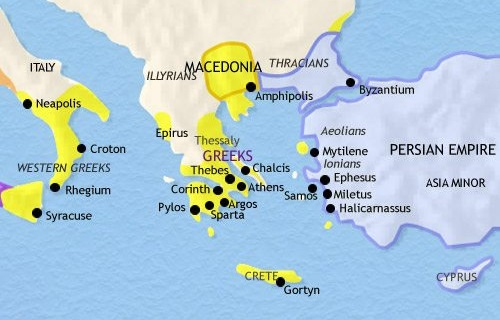
\includegraphics[scale=0.85]{greece500bc.jpg}\par
	Greek Territory c.\,500\BC{}% from \href{http://www.timemaps.com}{timemaps.com}
\end{center}

Greek mathematics is part of a much wider development of science and philosophy encompassing a change of emphasis from practicality to abstraction. One reason for this was the Greek blending of religion/mysticism with natural philosophy: philosophers wished to describe the natural world while preserving the idea of perfection/logic in the gods' design.\smallbreak

Early Greek inquiry into natural phenomena was encouraged through the personification of nature (e.g., sky = man, earth = woman). By 600\BC, philosophers were attempting to describe such phenomena in terms of natural predictable causes and structures. For example, some viewed matter as being comprised of the `four elements' (fire, earth, water, air); combined in the correct proportions\ldots While the \emph{system} was seen as divinely-designed, reliance on the whims of the gods was discouraged.\smallbreak

While the Greeks certainly used mathematics for practical purposes, philosophers idealized logic and were unhappy with approximations. This led to the development of \emph{axiomatics, theorems} and \emph{proof,} concepts for which there is scant pre-Greek evidence. Indeed ancient Greek is the source of three words of critical importance:\vspace{-3pt}
\begin{description}\itemsep0pt
	\item[]\emph{Mathematics} comes from \emph{mathematos} (\tgrk{μαθήματoς}), meaning knowledge or learning; the term covered essentially anything that might be taught in Greek schools.
	\item[]\emph{Geometry} literally means \emph{earth-measure}.\vspace{-6pt}
	\begin{description}\itemsep0pt
	\item[]\emph{Gi} (\tgrk{γη}) dates from pre-5\th{} century \!\BC{}, meaning \emph{land, earth} or \emph{soil.} Capitalized (\tgrk{Γη}) it could refer to the \emph{Earth} (as a goddess).
	\item[]\emph{Metron} (\tgrk{μέτρoν}) was a \emph{weight} or \emph{measure}, a \emph{dimension}  (length, width, etc.), or the \emph{metre} (rhythm) in music.
	\end{description}\vspace{-6pt}
	\item[]\emph{Theorem} comes from \emph{theoreo} (\tgrk{θεώρέω}), meaning `I contemplate,' or `consider.' In a mathematical context this become \emph{theorema} (\tgrk{θεώρημα}), a proposition to be proved.
\end{description}

Ancient Greece had several schools, mostly private and open only to men. %As an example of how education hasn't changed much in 2500 years, consider a quote from Isocrates (c.\,400\BC):
% \begin{quote}
% If it does no other good, the teaching of mathematics keeps the young out of mischief and the study of it helps to train one's mind and sharpen one's wits.
% \end{quote}
Typically arithmetic was taught until age 14, followed by geometry  and astronomy until age 18. The most famous scholars of ancient Greece were the Athenian trio of Socrates, Plato and Aristotle\footnote{Each taught his successor; the birth of Socrates to the death of Aristotle covered 470--322\BC.} whose writings became central to the Western/Islamic  philosophical tradition. Plato's \emph{Academy} in Athens was a model for centuries of schooling, the centrality of geometry to the curriculum evidenced by the famous inscription above the entryway: ``Let none ignorant of geometry enter here.''


\boldsubsubsection{Enumeration}

The ancient Greeks had two primary forms of enumeration, both dating from around 800--500\BC.\smallbreak

In \emph{Attic Greek} (Attica = Athens) strokes were used for 1--4, while larger numerals used the first letter of the words for 5, 10, 100, 1000 and 10000. For example,
\begin{itemize}\itemsep0pt
  \item \tgrk{Πεντε} (pente) is Greek for five, whence \tgrk{Π} denoted the number 5.
	\item \tgrk{Δεκα} (deca) means ten, so \tgrk{Δ} represented 10.
	\item \tgrk{Η} (hekaton), \tgrk{Χ} (khilias) and \tgrk{Μ} (myrion/myriad) denoted 100, 1000 and 10000 respectively.
	\item Combinations produced larger numbers, similar to Roman numerals, e.g., \tgrk{ΧΗΗΠ}$||=1207$.
\end{itemize}

\begin{minipage}[t]{0.69\linewidth}\vspace{-5pt}
	\emph{Ionic Greek} (Ionia = mid Anatolian coast) numerals used the Greek alphabet, an approach they possibly copied from the Egyptian hieratic method. Larger numbers used a left subscript mark (e.g., comma) to denote thousands and/or \tgrk{Μ} (with superscripts) for 10000, as in Attic Greek. For example,
	\[
		35298%,\!\lambda,\!\varepsilon\sigma\text{\tgrk{\textgreek{\qoppa}}}\eta %=\overset{\gamma}{\text{\tgrk{M}}},\!\varepsilon\sigma\text{\tgrk{\textgreek{\qoppa}}}\eta 
		=\text{\tgrk{,λ,εσ\textgreek{\qoppa}η}}
		= \overset{\text{\tgrk{γ}}}{\text{\tgrk{M}}}\!\text{\tgrk{,εσ\textgreek{\qoppa}η}} 
	\]
	The ancient Greek alphabet included three archaic symbols %{\selectlanguage{greek}Ϛ, Ϟ, Ϡ}
	\tgrk{\textgreek{\stigma,\ \qoppa,\ \sampi}}\ (stigma, qoppa, sampi), with which you're likely unfamiliar.
\end{minipage}
\hfill
\begin{minipage}[t]{0.3\linewidth}\vspace{-10pt}
	\flushright
	$\begin{array}{cc@{\qquad}cc@{\qquad}cc}
		1&\alpha&10&\iota&100&\rho\\
		2&\beta&20&\kappa&200&\sigma\\
		3&\gamma&30&\lambda&300&\tau\\
		4&\delta&40&\mu&400&\upsilon\\
		5&\varepsilon&50&\nu&500&\phi\\
		6&\text{\tgrk{\textgreek{\stigma}}}&60&\xi&600&\chi\\
		7&\zeta&70&o&700&\psi\\
		8&\eta&80&\pi&800&\omega\\
		9&\theta&90&\text{\tgrk{\textgreek{\qoppa}}}&900&\text{\tgrk{\textgreek{\sampi}}}
	\end{array}$
\end{minipage}
\medbreak


Eventually a bar was placed over numbers to distinguish them from words (e.g. $\overline{\text{\tgrk{ξθ}}}=89$). Modern practice is to place a \emph{keraia} (similar to an apostrophe) at the end of a number: thus $35298=\text{\tgrk{\greeknumeral{35298}}}$.  The Greeks also used Egyptian fractions, denoting reciprocals with an accent over the symbol: e.g., $\acute{\text{\tgrk{θ}}}=\frac 19$. The use of Egyptian fractions persisted in Europe well into the middle ages.\medbreak

Both the Attic and Ionic systems were fine for record-keeping but terrible for calculations! Later Greek mathematicians adapted the Babylonian sexagesimal system for calculation purposes, helping cement its modern use of in astronomy, navigation and time-keeping.


\begin{exercises}{}{}
	\exstart State the number 1789 in both Attic and Ionic notation.
	\begin{enumerate}\setcounter{enumi}{1}
	  \item%[2-2]
	  Represent $\frac 89$ as a sum of distinct unit fractions (Egyptian style). Express the result in (Ionic) Greek notation.\par
	  (\emph{The answer to this problem is non-unique})
	  
	  \item%[2-4]
	  For tax purposes, the Greeks often approximated the area of a quadrilateral field by multiplying the averages of the two pairs of opposite sides. In one example, the two pairs of opposite sides were given as
	  \begin{gather*}
	  a=\frac 14+\frac 18+\frac 1{16}+\frac 1{32}\quad\text{opposite}\quad c=\frac 18+\frac 1{16},\quad\text{and,}\\
	  b=\frac 12+\frac 14+\frac 18\quad\text{opposite}\quad d=1
	  \end{gather*}
	  where the lengths are in fractions of of a \emph{schonion,} a measure of approximately 150 feet. Find the average of $a$ and $c$, the average of $b$ and $d$, and thus the approximate area of the field in square \emph{schonion.} The taxman then rounds the answer up to collect a little more tax!
	\end{enumerate}
\end{exercises}

\clearpage



\subsection{Pre-Euclidean Greek Mathematics}

Euclid's \emph{Elements} (c.\,300\BC) forms a natural break point in Greek mathematics, since much of what came before was subsumed by it. In this section, we consider the contributions of several pre-Euclidean mathematicians. There are very few sources for Greek mathematics \& philosophy before 400\BC{}, so almost everything is inferred from the writings and commentaries of others.\footnote{For instance, most of our knowledge of Socrates comes from the voluminous writings of Plato and Aristotle. The earliest known Greek textbook/compilation (\emph{Elements of Geometry}) was written around 430\BC{} by Hippocrates of Chios; no copy survives, though most of its material probably made it into Book I of Euclid.}\vspace{-5pt}

\boldinline{Thales of Miletus (c.\,624--546\BC)}

One of the first people known to state abstract general principles, Thales was a trader based in Miletus, a city-state in Anatolia. He travelled widely and was likely exposed to mathematical ideas from all round the Mediterranean. Here are some statements at least partly attributed to Thales:\vspace{-3pt}
\begin{itemize}\itemsep0pt
  \item The angles at the base of an isosceles triangle are equal.
  \item Any circle is bisected by its diameter.
  \item A triangle inscribed in a semi-circle is right-angled (still known as Thales' Theorem).
\end{itemize}

\begin{minipage}[t]{0.79\linewidth}\vspace{-10pt}
	Thales' major development is \emph{generality}: his propositions concern \emph{all} triangles, circles, etc. The Babylonians/Egyptians observed such results in examples, but we have little indication that they believed these could be discerned by pure reason. Thales' reasoning was almost certainly visual. As an example of typical geometric reasoning of the period, by 425\BC{} Socrates could describe how to halve/double the area of a square by joining the midpoints of edges.
\end{minipage}
\hfill
\begin{minipage}[t]{0.2\linewidth}\vspace{-8pt}
  \flushright
  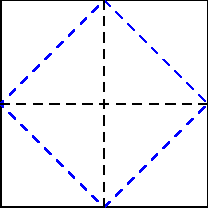
\includegraphics[scale=0.85]{greece-socratessquare}
\end{minipage}
\vspace{-5pt}



\boldinline{Pythagoras of Samos (c.\,572--497\BC)}

Like Thales, Pythagoras travelled widely, eventually settling in Croton (southeast Italy) where he founded a school lasting 100 years after his death. It is believed that Plato learned much of his mathematics from a Pythagorean named Archytas.\smallbreak
The Pythagoreans practiced a mini-religion with ideas out of the mainstream of Greek society.\footnote{They were vegetarians, believed in the transmigration of souls, and accepted women as students; controversial indeed!} One of their mottos, ``All is number,'' emphasised their belief in the centrality of pattern and proportion. The following quote\footnote{Van der Waerden, \emph{Science Awakening} pp 92--93} gives some flavor of the Pythagorean way of life.
\begin{quote}
  After a testing period and after rigorous selection, the initiates of this order were allowed to hear the voice of the Master [Pythagoras] behind a curtain; but only after some years, when their souls had been further purified by music and by living in purity in accordance with the regulations, were they allowed to see him. This purification and the initiation into the mysteries of harmony and of numbers would enable the soul to approach [become] the Divine and thus escape the circular chain of re-births.
\end{quote}

The Pythagoreans were particularly interested in musical harmony and the relationship of such to number. For instance, they related intervals in music to the ratios of lengths of vibrating strings:\vspace{-3pt}
\begin{itemize}\itemsep0pt\phantomsection\label{pg:pythagtuning}
  \item Identical strings whose lengths are in the ratio 2:1 vibrate an \emph{octave} apart.
  \item A \emph{perfect fifth} corresponds to the ratio 3:2.
  \item A \emph{perfect fourth} corresponds to the ratio 4:3.
\end{itemize}\vspace{-3pt}
The use of these intervals to tune musical instruments is still known as \emph{Pythagorean tuning.}
\goodbreak

Theorems 21--34 in Book IX of Euclid's \emph{Elements} are Pythagorean in origin. For instance:

\begin{thm*}{}{}
  {\normalfont\textbf{(IX\,.21)}}\lstsp A sum of even numbers is even.\par\vspace{-8pt}
  \begin{itemize}
    \item[]{\normalfont\textbf{(IX\,.27)}}\lstsp Odd less odd is even.
  \end{itemize}
\end{thm*}

The Pythagoreans also studied perfect numbers, those which equal the sum of their proper divisors (e.g. $6=1+2+3$), and they seem to have observed the following.

\begin{thm*}{IX.\,36}{}
	If $2^n-1$ is prime then $2^{n-1}(2^n-1)$ is perfect.
\end{thm*}

They moreover considered square and triangular numbers ($\frac 12m(m+1)$) and tried to express geometric shapes as numbers, in service of their belief that all matter could be formed from basic shapes.%Cultish the Pythagoreans may have been, but they discovered many things!
\vspace{-5pt}



\boldinline{Incommensurability and Pythagoras' Theorem}

As with other ancient cultures, the only numbers in Greek mathematics were \emph{positive integers.} These were used to \emph{compare} lengths/sizes of objects.

\begin{defn*}[lower separated=false, sidebyside, sidebyside align=top seam, sidebyside gap=0pt, righthand width=0.19\linewidth]{}{}
	Lengths are in the ratio $m$\,:\,$n$ if some \textcolor{blue}{sub-length} divides exactly $m$ times into the first and $n$ times into the second.\par
	Lengths are \emph{commensurable} if some sub-length divides exactly into both.
	\tcblower
	\flushright
	\begin{tabular}{c@{}}
		
\includegraphics{similar-ruler}\\
		Ratio 3\,:\,2
	\end{tabular}
\end{defn*}

While modern mathematics has no problem with \emph{irrational ratios} (e.g., the diagonal of a square to its side is $\sqrt 2$\,:\,1), this conflicted with the core Pythagorean belief that \emph{any two lengths were commmensurable.} Identifying lengths with real numbers, this belief may be restated in modern language:
\[
	\forall \underline{m},\underline n\in\R^+,\ \exists \underline\ell\in\R^+,\ \exists a,b\in\N,\ \text{such that}\ \underline m=a\underline\ell\ \text{and}\ \underline n=b\underline\ell
\]
This is complete nonsense for it insists that every ratio of real numbers $\frac{\underline m}{\underline n}=\frac ab$ must be \emph{rational}!\smallbreak

The Pythagorean commensurability supposition stems from their basic tenets: all is number (lengths represented numerically) and that the design of the gods be perfect (numbers are integers). The discovery of incommensurable ratios produced something of a crisis; a possibly apocryphal story states that a disciple named Hippasus (c.\,500\BC) was set adrift at sea as punishment for its revelation.\smallbreak %Nevertheless, it is generally accepted that the Pythagoreans provided the first evidence of the existence of irrational numbers in the form of incommensurable lengths.

By 340\BC, however, the Greeks were happy to state that incommensurable lengths exist.

\begin{thm*}{Aristotle}
	If the diagonal and side of a square are commensurable, then odd numbers equal even numbers.
\end{thm*}

\begin{proof}[Inferred proof]
	In Socrates' doubled-square, suppose that side\,:\,diagonal $=a$\,:\,$b$; \ these are integers!\par
	\begin{minipage}[t]{0.8\linewidth}\vspace{-5pt}
		Assume at least one of $a$ or $b$ is odd, else the common sub-length may be doubled. The larger square is twice the smaller, whence the square numbers have ratio
		\[
			b^2:a^2=2:1
		\]
		It follows that $b^2$ is even and thus divisible by 4, whence $a^2$ is also even, and both $a,b$ are even. Whichever of $a,b$ was odd is also even: contradiction!
	\end{minipage}
	\hfill
	\begin{minipage}[t]{0.18\linewidth}\vspace{-8pt}
		\flushright
		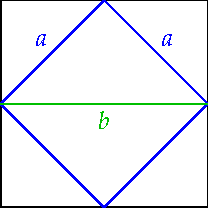
\includegraphics[scale=0.8]{greece-socratessquare2}
	\end{minipage}
\end{proof}
Note the similarity of this argument to the modern proof of the irrationality of $\sqrt 2$.\goodbreak

While there is no evidence that the Pythagoreans ever provided a correct proof of their famous Theorem, one argument possibly attributable to them used the idea of commensurability.

\begin{minipage}[t]{0.67\linewidth}\vspace{0pt}
	\begin{proof}[`Proof' of Pythagoras' Theorem]\label{pg:pythwrong}
		Label the right triangle $a,b,c$ where $c$ is the hypotenuse and drop the altitude to the hypotenuse. Let $d$ be the length shown. Similar triangles tell us that
		\[
			a:d=c:a\implies a^2:ad=cd:ad\implies a^2=cd
		\]
		Thus the square on $a$ has the same area as the rectangle below the $d$-side of the hypotenuse. Repeat the calculation on the other side to obtain $b^2=c(c-d)$, and sum to complete the proof.
	\end{proof}

	Since the only \emph{numbers} were integers, the symbols $a,b,c,d$ are \emph{integer multiples} of an assumed common sub-length. This restriction completely destroys the generality of the argument.
\end{minipage}
\hfill
\begin{minipage}[t]{0.32\linewidth}\vspace{0pt}
	\flushright
	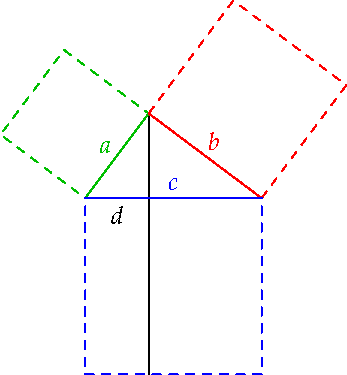
\includegraphics[scale=0.85]{greece-pthag-false}\label{pthagorig}
\end{minipage}
\smallbreak

The organization of Book I of the \emph{Elements} make clear that its primary goal was to provide a rigorous proof of Pythagoras' Theorem which did not depend on the flawed notion of commensurability. With our modern understanding of real numbers and continuity, there is nothing wrong with the above.%\vspace{-5pt}




\boldinline{Theaetetus of Athens (417--369\BC)}\def\ul{\underline}

Theaetetus is likely the source for much of the most difficult part (Books VII \& X) of the \emph{Elements.} His essential definition of (in)commensurability comes from applying what is now known as the Euclidean algorithm to line segments. 

\begin{defn*}{}{}
	Let $\ul a>\ul b$ be lengths/segments\footnotemark{} ($\ul a$ is longer than $\ul b$). Repeatedly the division algorithm: 
	\begin{align*}
		\ul a&=q_1\ul b+\ul r_1\qquad &&\ul r_1<\ul b&&\hspace*{100pt}\tag{$\exists q_1\in\N_0$ and a length $\ul r_1<\ul b$}\\
		\ul b&=q_2\ul r_1+\ul r_2\qquad &&\ul r_2<\ul r_1\\
		\ul r_1&=q_3\ul r_2+\ul r_3\qquad &&\ul r_3<\ul r_2
	\end{align*}
	We say that $\ul a$ and $\ul b$ are \emph{commensurable} if the algorithm terminates: some remainder $\ul r_n$ divides exactly into $\ul r_{n-1}$. Otherwise $\ul a$ and $\ul b$ are \emph{incommensurable.}\smallbreak
	Ratios are \emph{equal} $\ul a:\ul b=\ul c:\ul d$ precisely when the sequences of quotients in the algorithm are equal.
\end{defn*}

\footnotetext{\emph{Only} the quotients $q_k$ need be integers, everything underlined is a \emph{segment.}}

If $\ul a$ and $\ul b$ are commensurable, then $\ul r_n$ is their \emph{greatest common sub-length}. If we write $\ul a=a\ul r_n$ and $\ul b=b\ul r_n$ for integers $a,b$, and rewrite the algorithm in the modern fashion, the result is the standard Euclidean algorithm computation of $\gcd(a,b)=1$.

\boldinline{Example 1}
$37:13=148:52$ since we obtain the same sequence of quotients $(2,1,5,2)$:
\begin{align*}
	\ul{37}&=2\cdot\ul{13}+\ul{11}\qquad &\ul{148}&=2\cdot\ul{52}+\ul{44}\\
	\ul{13}&=1\cdot\ul{11}+\ul{2}\qquad &\ul{52}&=1\cdot\ul{44}+\ul{8}\\
	\ul{11}&=5\cdot\ul{2}+\ul{1}\qquad &\ul{44}&=5\cdot\ul{8}+\ul{4}\\
	\ul{2}&=2\cdot\ul{1}\qquad &\ul{8}&=2\cdot\ul{4}
\end{align*}

\goodbreak

\boldinline{Example 2}\phantomsection\label{ex:theaetetus} We sketch a proof that the side $AB$ and diagonal $AC$ of a regular pentagon $ABCDE$ are incommensurable.\par
\begin{minipage}[t]{0.65\linewidth}\vspace{-5pt}
	\begin{enumerate}\itemsep0pt
	  \item Prove that $\triangle BAG$ is isosceles ($\angle GFK=\frac 35\cdot\ang{180}=\ang{108}$\ldots).
	  \item Take $a=\nm{AC}$ and $b=\nm{AB}=\nm{AG}$. The first line of the algorithm now reads
	  \[
	  	\nm{AC}=\nm{AG}+\nm{GC}=\nm{AB}+\nm{GC}
	  \]
	  so we write $\underline a=q_1\underline b+\underline r_1$ where $r_1=\nm{GC}$ and $q_1=1$.
	  \item Since $\nm{GC}=\nm{AF}$, the second line of the algorithm reads
	  \[
	  	\nm{AG}=\nm{AF}+\nm{FG}=\nm{GC}+\nm{FG}
	  \]
	  so that we again have a quotient of $q_2=1$.
	\end{enumerate}
\end{minipage}
\hfill
\begin{minipage}[t]{0.34\textwidth}\vspace{-5pt}
	\flushright
	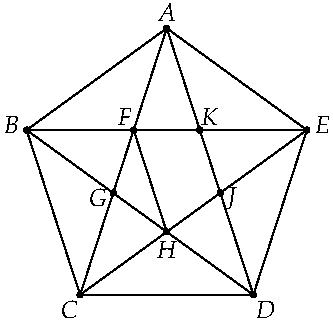
\includegraphics[scale=0.9]{greece-pentagonincomm}
\end{minipage}
	
	
\begin{enumerate}\setcounter{enumi}{3}
	\item Appealing to congruent isosceles triangles $\triangle DCG\cong\triangle EHF$ we see that $\nm{GC}=\nm{FH}$ is the diagonal of the interior regular pentagon. The third line of the algorithm is therefore the same as the first: we are back to considering the ratio of the diagonal to the side of a regular pentagon. The algorithm therefore continues forever with all quotients being 1.
\end{enumerate}


\boldinline{Example 3}

In modern language, the diagonal to the side of a square is the incommensurable ratio $\sqrt 2:1$. We apply Theaetetus' algorithm:
\begin{gather*}
	\underline{\sqrt 2}=1\cdot \underline 1+(\underline{\sqrt 2-1})\\
	\underline 1=2\cdot(\underline{\sqrt 2-1})+(\underline{3-2\sqrt 2})
\end{gather*}
Observe that $3-2\sqrt 2=(\sqrt 2-1)^2$, whence the second line reads $1=2x+x^2$. The following lines in the algorithm may therefore be obtained by repeatedly multiplying by $x$:
\[
	x=2x^2+x^3,\quad x^2=2x^3+x^4,\text{etc.,}
\]
resulting in a never-ending sequence\footnote{If you're interested in number theory, investigate the relationship of Theaetetus' algorithm to continued fractions\ldots} of quotients: $1,2,2,2,2,2,\ldots$
	
% \goodbreak



\boldinline{Eudoxus of Knidos (c.\,390--337\BC)}\phantomsection\label{pg:eudoxus}

Eudoxus was arguably the most prolific of the pre-Euclidean mathematicians. Apart from attending and perhaps teaching at Plato's academy, he is famous for explaining how to calculate with ratios of lengths (segments). For example:

\begin{defn*}{}{}
	$A:B>C:D$ if there exist positive integers $m,n$ such that $mA>nB$ and $mC\le nD$.
\end{defn*}

At first glance it appears as if Eudoxus is telling us how to compare \emph{rational} numbers; if $A,B,C,D$ are integers, we see that
\[
	\frac AB>\frac nm\ge \frac CD
\]
which is trivially satisfied by taking $m=D$ and $n=C$. However, if $A,B,C,D$ were interpreted as \emph{segments} rather than integers this is much more useful. Building on the work of Theaetetus, his mathematics told the Greeks how to approximate incommensurable ratios with rational numbers.


\boldinline{Examples}
\exstart To see that $13:3>17:4$, simply choose $m=4$ and $n=17$ to obtain
  \[4\cdot 13=52>51=3\cdot 17\]

\begin{enumerate}\setcounter{enumi}{1}
  \begin{minipage}[t]{0.68\linewidth}\vspace{-10pt}
    \item We show that the side\,:\,diagonal of a square is greater than 1\,:\,2; equivalently, the diagonal is less than twice the side.\par
    See the picture, where the side\,:\,diagonal $=A:B$. Choosing $m=D=2$ and $n=C=1$, we see that
  	\[
  		mA=2A>B=nB \tag{diag $>$ side of large square}
  	\]
  	In modern language, this is merely $\frac 1{\sqrt 2}>\frac 12$.
  \end{minipage}
  \hfill
  \begin{minipage}[t]{0.31\linewidth}\vspace{-10pt}
  	\flushright
  	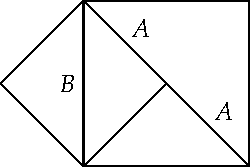
\includegraphics{greece-eudoxus}
  \end{minipage}
\end{enumerate}


\boldinline{Zeno of Elea (c.\,450\BC)}\phantomsection\label{pg:zeno}

%No discussion of pre-Euclidean mathematics would be complete without Zeno. 
While not strictly a mathematician, Zeno's arguments have become essential parts of the discussion of the infinite and the infinitesimal. These provided fodder for philosophers for thousands of years and lie at the heart of the controversy surrounding the development of calculus. Here are two of the most famous:
\begin{description}\itemsep0pt
  \item[\normalfont\emph{Achilles and Tortoise}] Achilles chases a Tortoise. After time $t_0$, Achilles reaches the Tortoise's starting position, but the Tortoise has moved on. After another time $t_1$, Achilles reaches the Tortoise's second position; again the Tortoise has moved. In this manner Achilles spends $t_0+t_1+t_2+\cdots$ in the chase. Zeno's paradoxical conclusion is that Achilles never catches the Tortoise.\par
  The resolution is that the total duration can be finite, even though it be split into infinitely many subintervals of time; this idea is at the heart of the modern notion of \emph{infinite series.}
  %\item If any two lengths are commensurable, then there must be a smallest unit of space? Everything made up of elements, so can't be infinitely small?????? FIX PHRASING
  \item[\normalfont\emph{Arrow paradox}] An arrow is shot from a bow. At any given instant the arrow doesn't move. If time is made up of instants, then the arrow never moves.\par
  This time Zeno debates the the idea that a finite time period can be considered as a sum of infinitesimal instants. The modern resolution involves the \emph{integral.}
\end{description}


\boldinline{Constructions and Geometry}\phantomsection\label{pg:construction}

By the middle of the 5\th{} century \!\BC, Greek mathematicians were solving geometric problems using \emph{ruler-and-compass} (peg-and-cord) constructions. This approach perhaps came to Greece from India, or could have arisen organically. Constructions were based on three rules, which became the first three postulates (axioms) of Book I of Euclid's \emph{Elements.}\vspace{-1pt}
\begin{enumerate}\itemsep0pt
  \item One may join two given points by with straight line segment.
  \item Any segment may be extended indefinitely.
  \item Given a center and radius, one may draw a circle.
\end{enumerate}\vspace{-1pt}
Theorems were often stated as \emph{problems}: e.g., \emph{to bisect a given angle.} A proof provided first a \emph{construction,} then an argument justifying that the construction really had solved the problem.\smallbreak 

By the time of Euclid, the Greeks knew how to construct an equilateral triangle, a square and a regular pentagon in a given circle: here is a construction of a pentagon.\footnote{Theorem IV.\,11 of the \emph{Elements} presents a less practical construction. Ours follows from Theorem XIII.\,10: if a regular pentagon, hexagon and decagon are inscribed in a circle, then their sides form a right-triangle.}

\begin{minipage}[t]{0.69\linewidth}\vspace{-8pt}
	\begin{enumerate}\itemsep0pt
	  \item Draw perpendicular diameters $\cl{AB}$ and $\cl{CD}$ and bisect $\cl{OA}$ at $M$.
	  \item Draw an arc centered at $M$ with radius $\nm{CM}$. Let $N$ be the intersection of this arc with $\cl{OB}$.
	  \item Draw an arc centered at $C$ with radius $\nm{CN}$. Let $R$ be the intersection of this arc with the original circle.
		\item Move $\nm{CR}$ around the circle to create a regular pentagon.
	\end{enumerate}
\end{minipage}
\hfill
\begin{minipage}[t]{0.3\linewidth}\vspace{-22pt}
	\flushright
	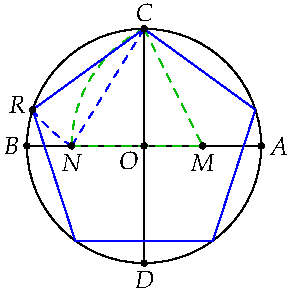
\includegraphics[scale=0.8]{greece-pentagon}
\end{minipage}
\smallbreak


A purely geometric proof of the validity of this construction is too difficult for us, but you can easily check it using a calculator, Pythagoras' and the cosine rule:  if the circle has radius 2, then
\begin{align*}
	\nm{CR}^2&=\nm{CN}^2=\nm{ON}^2+\nm{OC}^2=(\sqrt 5-1)^2+2^2=10-2\sqrt 5 =2^2+2^2-2\cdot 2\cdot 2\cos\ang{72}
\end{align*}\goodbreak

% The appearance of $\sqrt 5$ in this discussion relates to the golden ratio $\frac{1+\sqrt 5}2$ which is in fact the ratio of the diagonal to the side of the pentagon: exactly what Theaetetus was calculating on page \pageref{ex:theaetetus}. Pentagons and pentagrams were viewed as mystical by many ancient Greeks.\\

Construction problems have motivated mathematicians ever since. In 1796, Gauss (then 19) constructed a regular 17-gon. A classification of constructable regular polygons took until 1837.

\begin{thm*}{}{}
	A regular $n$-gon is constructable if and only if $n=2^kF_1\cdots F_r$ where $F_1,\ldots,F_r$ are distinct primes of the form $2^{(2^n)}+1$.
\end{thm*}

After the 17-gon, the next prime-sided constructable $n$-gon has $257=2^{2^3}+1$ sides!\smallbreak

By 400\BC, the Greeks were referencing the second and third \emph{impossible constructions of antiquity}:
\begin{enumerate}\itemsep0pt
  \item Trisecting a general angle.
  \item Doubling (the volume of) a given cube.
  \item Squaring a circle (construct a square with the same area as a given circle).\footnotemark
\end{enumerate}
It wasn't until the advent of field theory in the 1800s that these were indeed proved to be impossible using ruler-and-compass constructions.

\footnotetext{``You can't square that circle'' is now a metaphor for something that can't be done.}





\boldsubsubsection{Summary}

Several of the mathematical techniques in this section are difficult, and the results are technical. With practice, all should be accessible. It isn't important to become proficient with all of these ideas! Instead, by playing with them, you should develop an appreciation of two overarching points:
\begin{enumerate}
  \item Even before Euclid, the focus of Greek mathematics was more abstract and less practical than other ancient cultures (e.g., the Egyptians, Babylonians \& Chinese), in large part due to the influence of wider Greek philosophy and religion. The modern liberal arts ideal of learning for its own sake---to celebrate the beauty of knowledge and to expand the mind---is, to a large extent, a Greek inheritance. 
  \item By investigating mathematics abstractly, the ancient Greeks were already pondering fundamental mathematical questions and concepts, for instance: the relationship between \emph{number} and \emph{length}, continuity, irrationality, infinitesimals \& constructability.
%   \begin{itemize}
%     \item What is the relationship between \emph{number} and \emph{length}?
%     \item What are irrational numbers?
%     \item What is continuity?
%     \item Infinite series and integration.
%     \item Which geometric figures can we construct?
%   \end{itemize}
  Such ideas have stimulated mathematical research ever since. Indeed these particular issues would not rigorously be resolved until the development of modern analysis and algebra in the 1800s by luminaries such as Gauss, Cauchy and Riemann.
\end{enumerate}


\clearpage


\begin{exercises}{}{}
	\exstart %[2-12]
	Construct five Pythagorean triples using the formula $\bigl(n,\frac{n^2-1}2,\frac{n^2+1}2\bigr)$ where $n$ is odd. Construct five more using the formula $\bigl(m,\leg m2^2-1,\leg m2^2+1\bigr)$ where $m$ is even.%\vspace{-3pt}
	
	\begin{enumerate}\setcounter{enumi}{1}
	  \item Suppose $2^n-1=p$ is prime (its only positive divisors are itself and 1). List the positive divisors of $2^{n-1}(2^n-1)$ and hence prove Theorem IX.\,36.
	  
	  \item%[2-10]
	  Draw a \emph{picture} with dots to show that eight times any triangular number plus 1 makes a square, and that any odd square diminished by 1 becomes eight times a triangular number. That is:
	  \begin{enumerate}
	    \item[(a)] $8\cdot\frac 12m(m+1)+1$ is a perfect square.
	    \item[(b)] If $n$ is odd, then $n^2-1=8\cdot\frac 12m(m+1)$ for some $m$.
	  \end{enumerate}
	  
	  \item%[3-2]
	  Find a construction (using the \emph{ruler-and-compass} constructions) to bisect a given angle, and show that it is correct.
	 
	  \item%[3-16]
	  Sketch a construction inscribing a regular hexagon in a circle.\par
	  (\emph{Assume you can construct an equilateral triangle on a given segment---Thm I.\,1 of Euclid, pg.\,\pageref{pg:euclidI1}})
	  
		\item (A line-doubling paradox) \ One line has twice the length of another and so has \emph{more} points. However, there is a bijective correspondence between the points on these lines; the two lines therefore have the \emph{same number} of points.\par
		Explain the second observation. How can you resolve the paradox?
	
	
		\item The \emph{cycle of fifths} is a musical concept stating that twelve perfect fifths equals seven octaves (pg.\,\pageref{pg:pythagtuning}). State this claim \emph{numerically,} and show that it is a contradiction.\par
		(\emph{Hint: two strings are seven octaves apart if their lengths are in the ratio $2^7:1$})
		
		
		\item We use modern language to resolve Zeno's paradox of Achilles and the Tortoise. Suppose Achilles travels at speed $v_A$, the tortoise at speed $v_B<v_A$, and that the tortoise starts a distance $d$ ahead of Achilles.
		\begin{enumerate}
		  \item Prove that $t_n=\frac d{v_A}\left(\frac{v_T}{v_A}\right)^{n}$ for each positive integer $n$.
		  \item Compute $\sum_{n=0}^\infty t_n$ using the geometric series formula from calculus.
		  \item Verify the time-value computed in (b) as would a modern Physicist; by considering the motion of Achilles relative to the tortoise.
		\end{enumerate} 
		
	  
	  \item%[3-20]
		Use Theaetetus' definition of equal ratios to prove that $46:6=23:3$.
	  
	  
	  \item%[3-22]
	  (Hard)\lstsp A line of length 1 is divided at $x$ so that $\frac 1x=\frac x{1-x}$. Prove that 1 and $x$ are incommensurable. Indeed, show that $1:x$ is \emph{the same} as diagonal\,:\,side of a regular pentagon.\par
	  (\emph{Hint: the first line of the algorithm is $1=x+x^2$\ldots})
	  
	  
	  \item%[3-24]
	  (Hard)\lstsp Let $a>b$ and $c$ be \emph{positive lengths.} Use Eudoxus' definition to \emph{prove} that $c:b>c:a$.\par
	  (\emph{Hint: let $n$ be the smallest integer such that $n(a-b)\ge c$; its existence is the ``archimedean property''})
	\end{enumerate}
\end{exercises}


\clearpage



\subsection{Euclid and the \emph{Elements}}

\begin{minipage}[t]{0.70\linewidth}\vspace{-8pt}
	Euclid worked in the Library of Alexandria, named for the Greek general Alexander the Great who conquered Egypt in 323\BC. The Library was constructed around 320\BC{} as a means of organizing the knowledge of the world and for the demonstration of Greek power. Although it was seriously damaged on several occasions, the Library remained a center of scholarship until around \AD 500. Below is a map of the city around \AD 400: note the size and centrality of the \textcolor{red}{Library}.
\end{minipage}
\hfill
\begin{minipage}[t]{0.29\linewidth}\vspace{-25pt}
	\flushright
	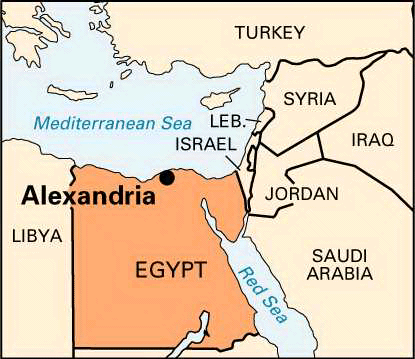
\includegraphics[scale=0.4]{geo-08-alex}
\end{minipage}\par

\begin{center}
	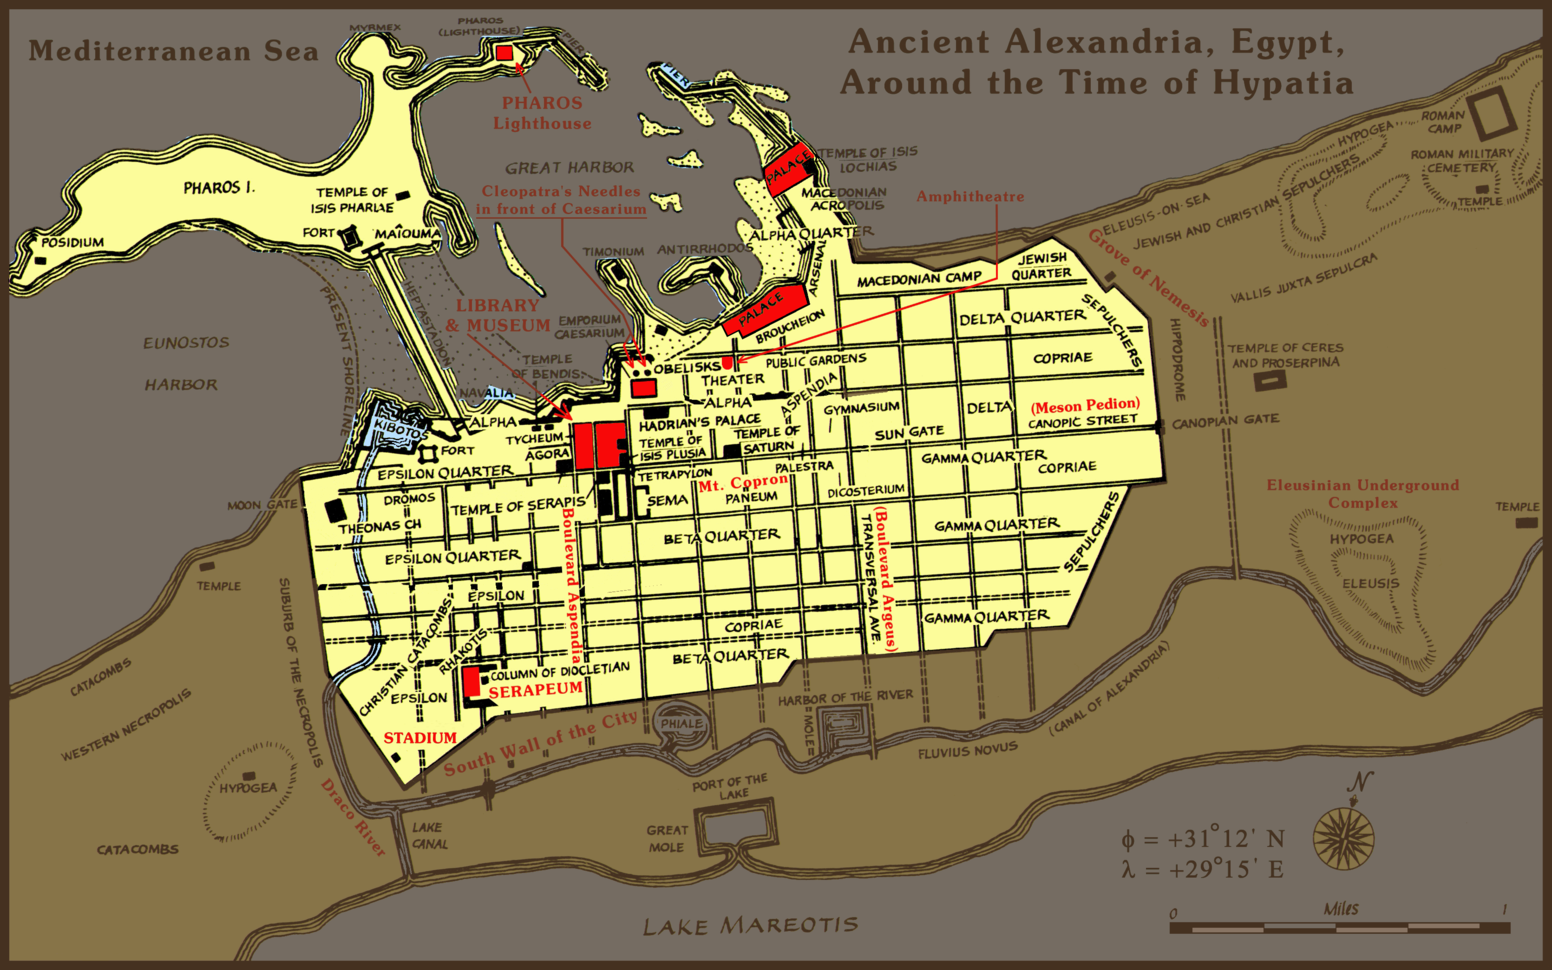
\includegraphics[scale=0.67]{geo-07-alexandria}
\end{center}

It is hard to argue against Euclid's \emph{Elements} (c.\,300\BC{}) as the most influential mathematics text ever produced. Likely a compilation of earlier mathematical work rather than a pure original, it was edited and added to over the centuries, eclipsing and subsuming other works. Particular import were the edits of Theon of Alexandria (c.\,\AD 400) and his daughter Hypatia, both prolific scholars in their own right. Due to edits such as these, the precise contents of the original are unknown.\smallbreak

Extant fragments date to around \AD 100. The earliest (almost) complete copy is from the the 9\th{} century; written in Greek and held at the Vatican, it is missing some of the edits of Theon \& Hypatia, thus demonstrating that multiple versions were in circulation.

\begin{center}
	\begin{minipage}[b]{0.45\linewidth}
		\centering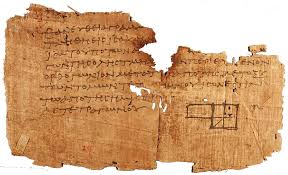
\includegraphics[scale=0.7]{euclid1}\\
		Earliest Fragment c.\,\AD 100
	\end{minipage}
	\begin{minipage}[b]{0.45\linewidth}
		\centering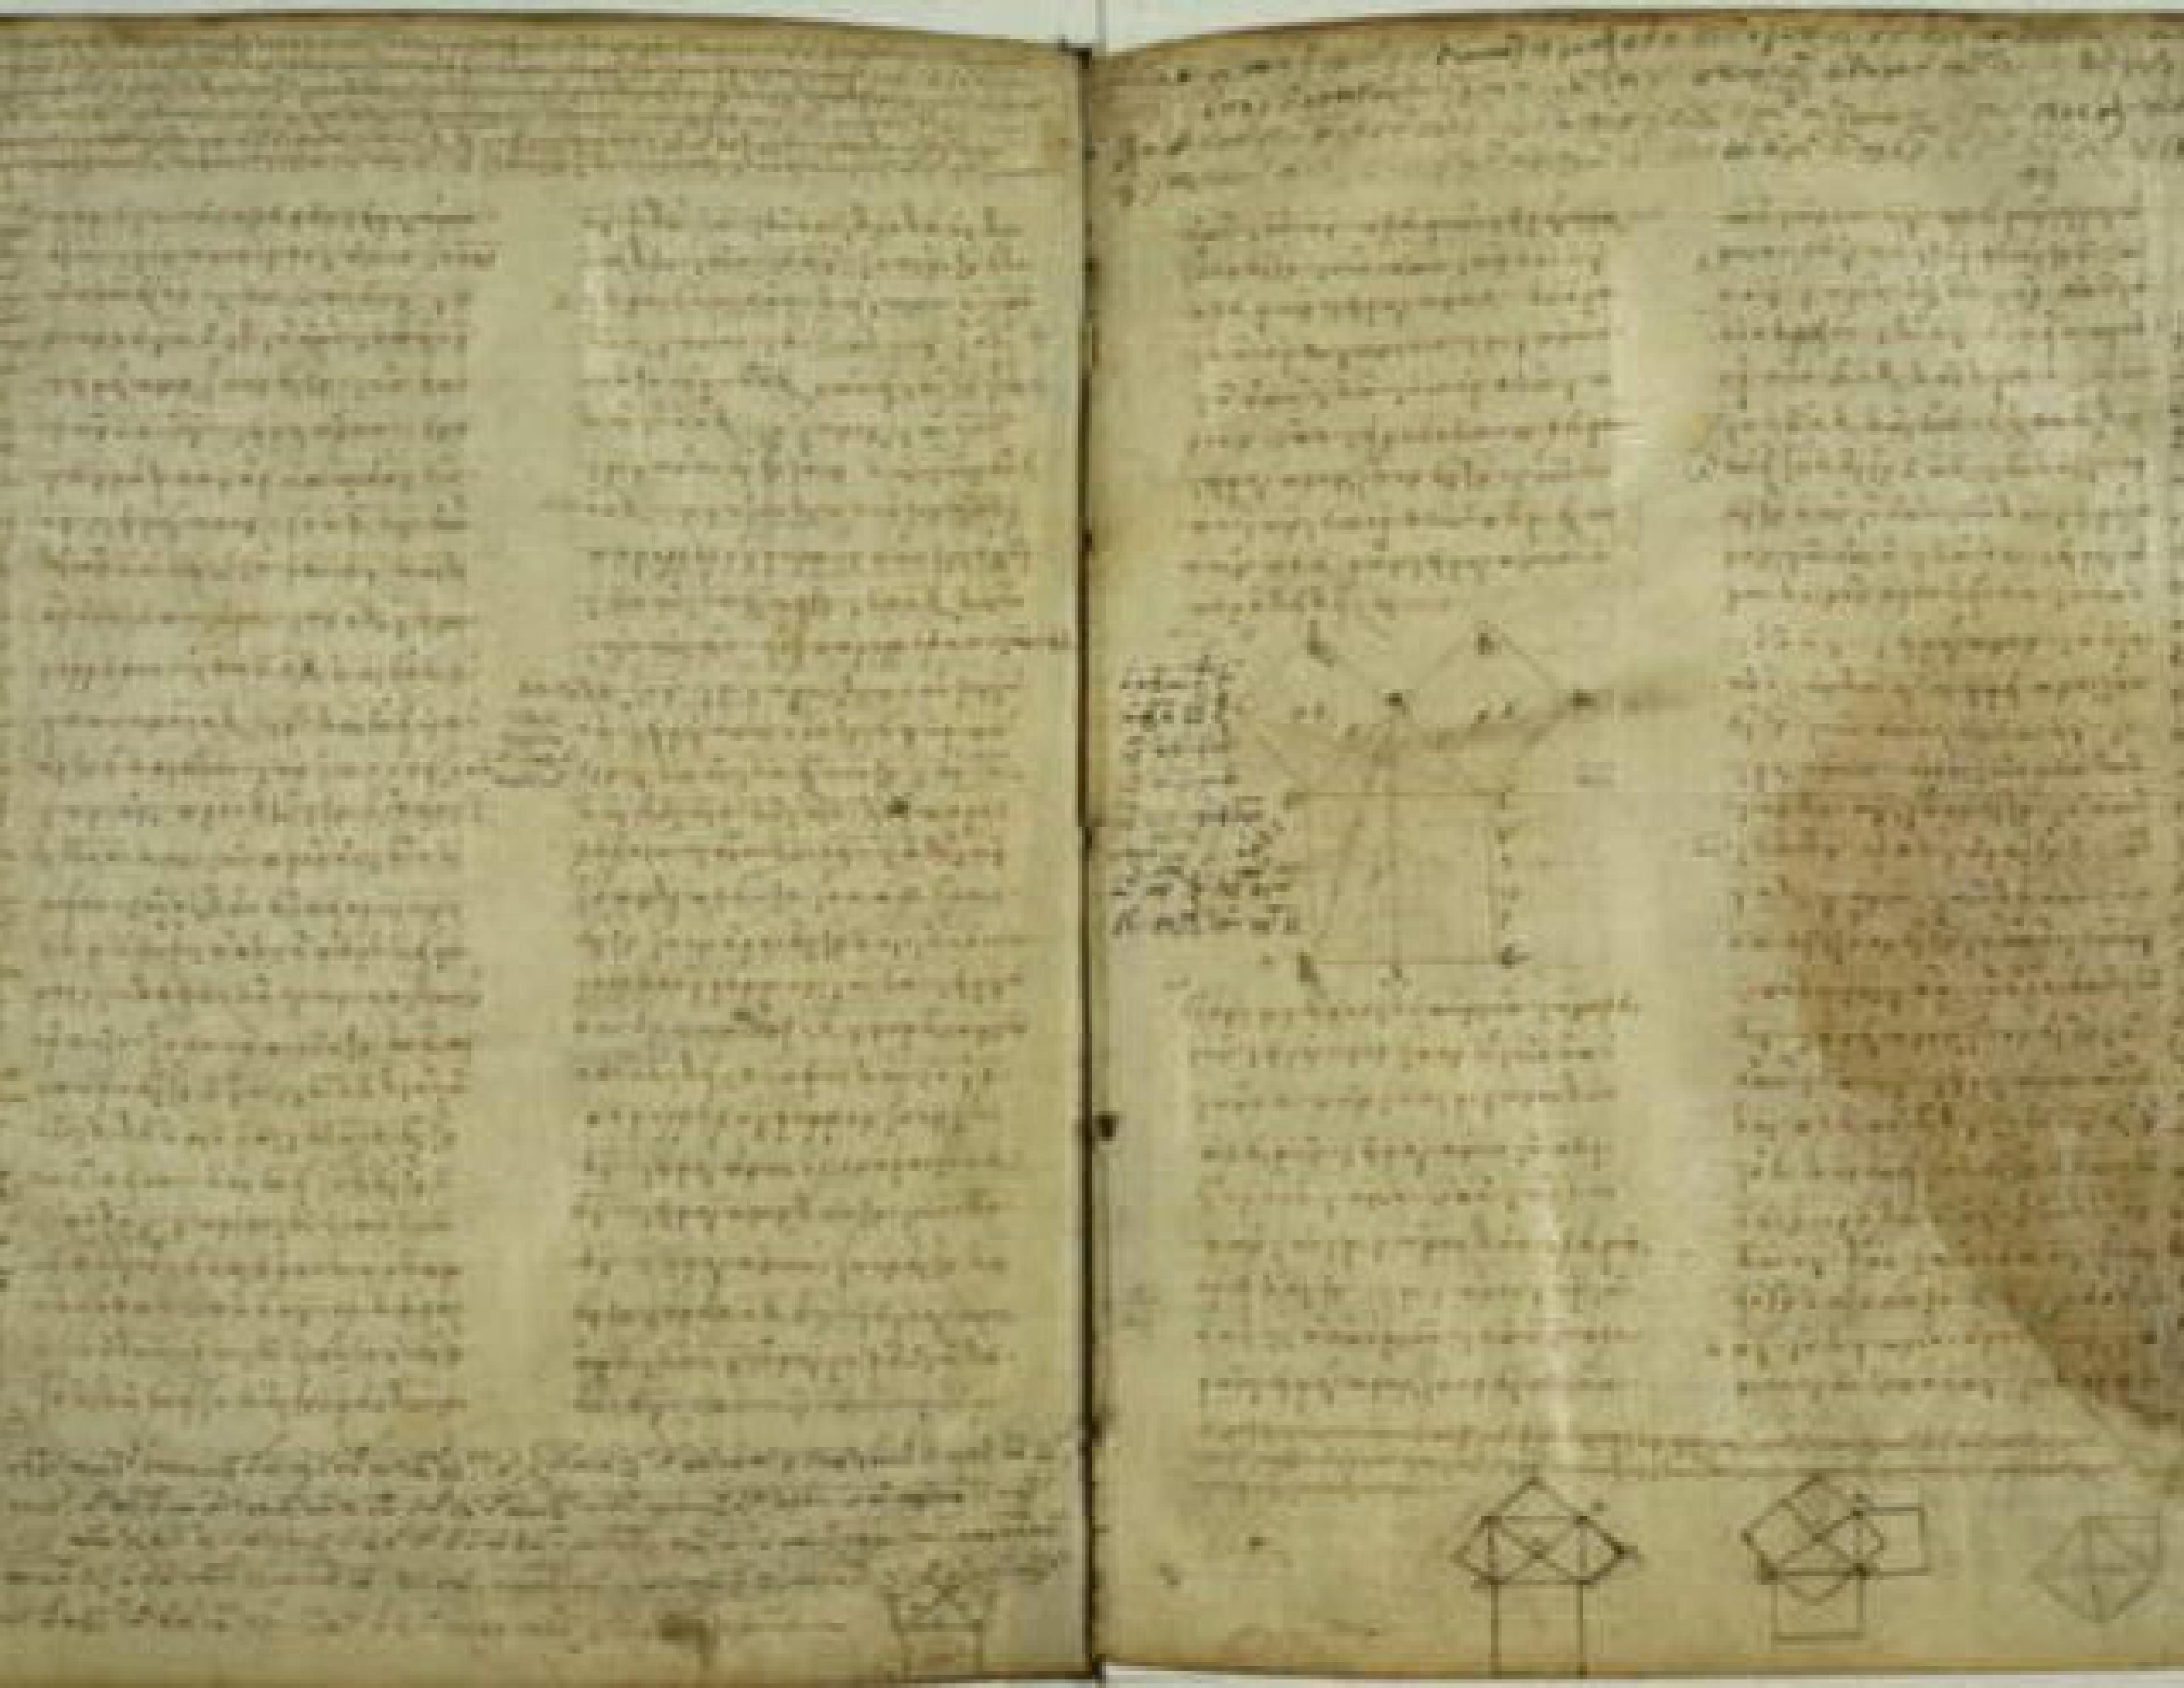
\includegraphics[scale=0.2]{euclid2}\\
		Full copy 9\th\,C
	\end{minipage}
\end{center}

\goodbreak

Until the mid 20\th{} century, some version of the \emph{Elements} would have been used as a high-school textbook in most western and middle-eastern countries. Many editions and variations have been produced, four of which are shown below:
\begin{center}
	\begin{minipage}[b]{0.683\linewidth}\vspace{0pt}
		\centering
		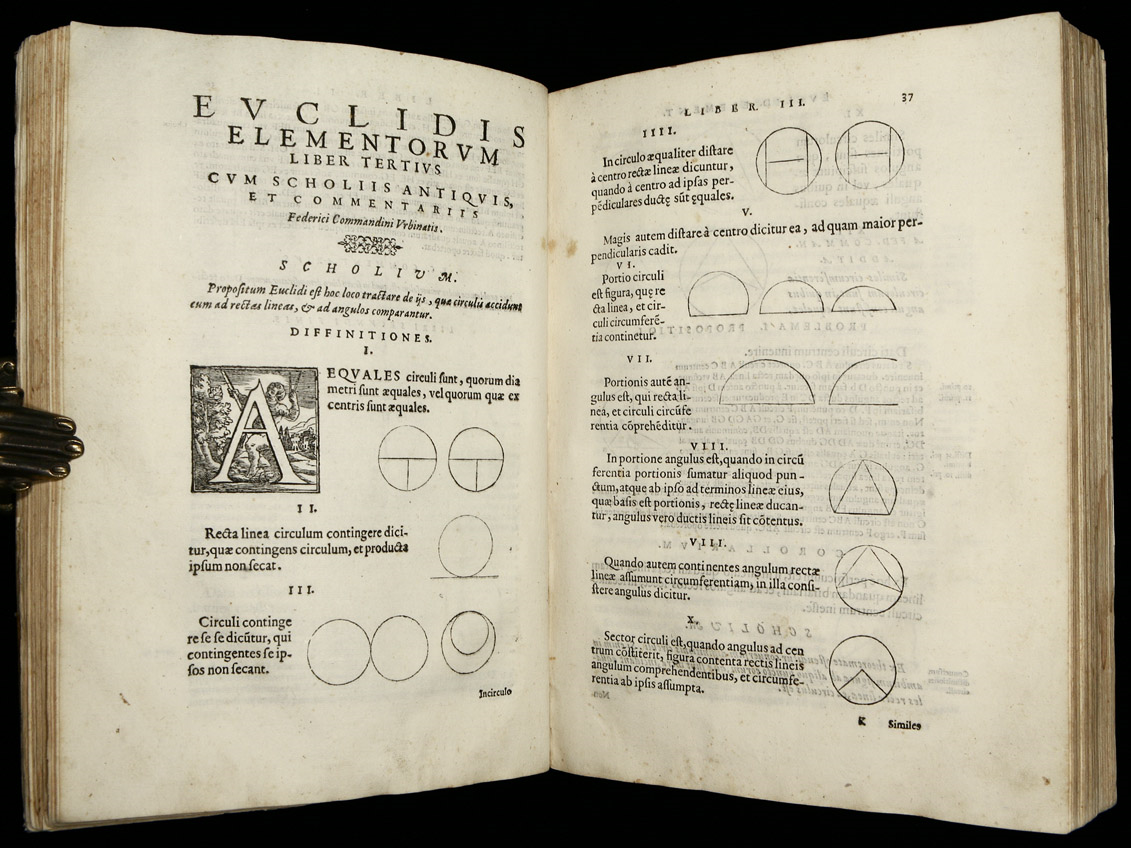
\includegraphics[width=0.95\linewidth]{geo-09-euclid}\\
		Latin translation, 1572
	\end{minipage}%
	\begin{minipage}[b]{0.317\linewidth}\vspace{0pt}
		\centering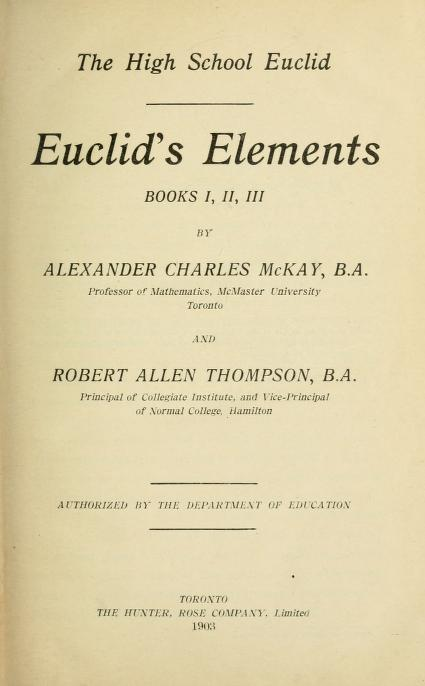
\includegraphics[width=0.95\linewidth]{euclid4}\\
		High School textbook, 1903
	\end{minipage}%
	\smallbreak
	\begin{minipage}[b]{0.67\linewidth}\vspace{0pt}
		\centering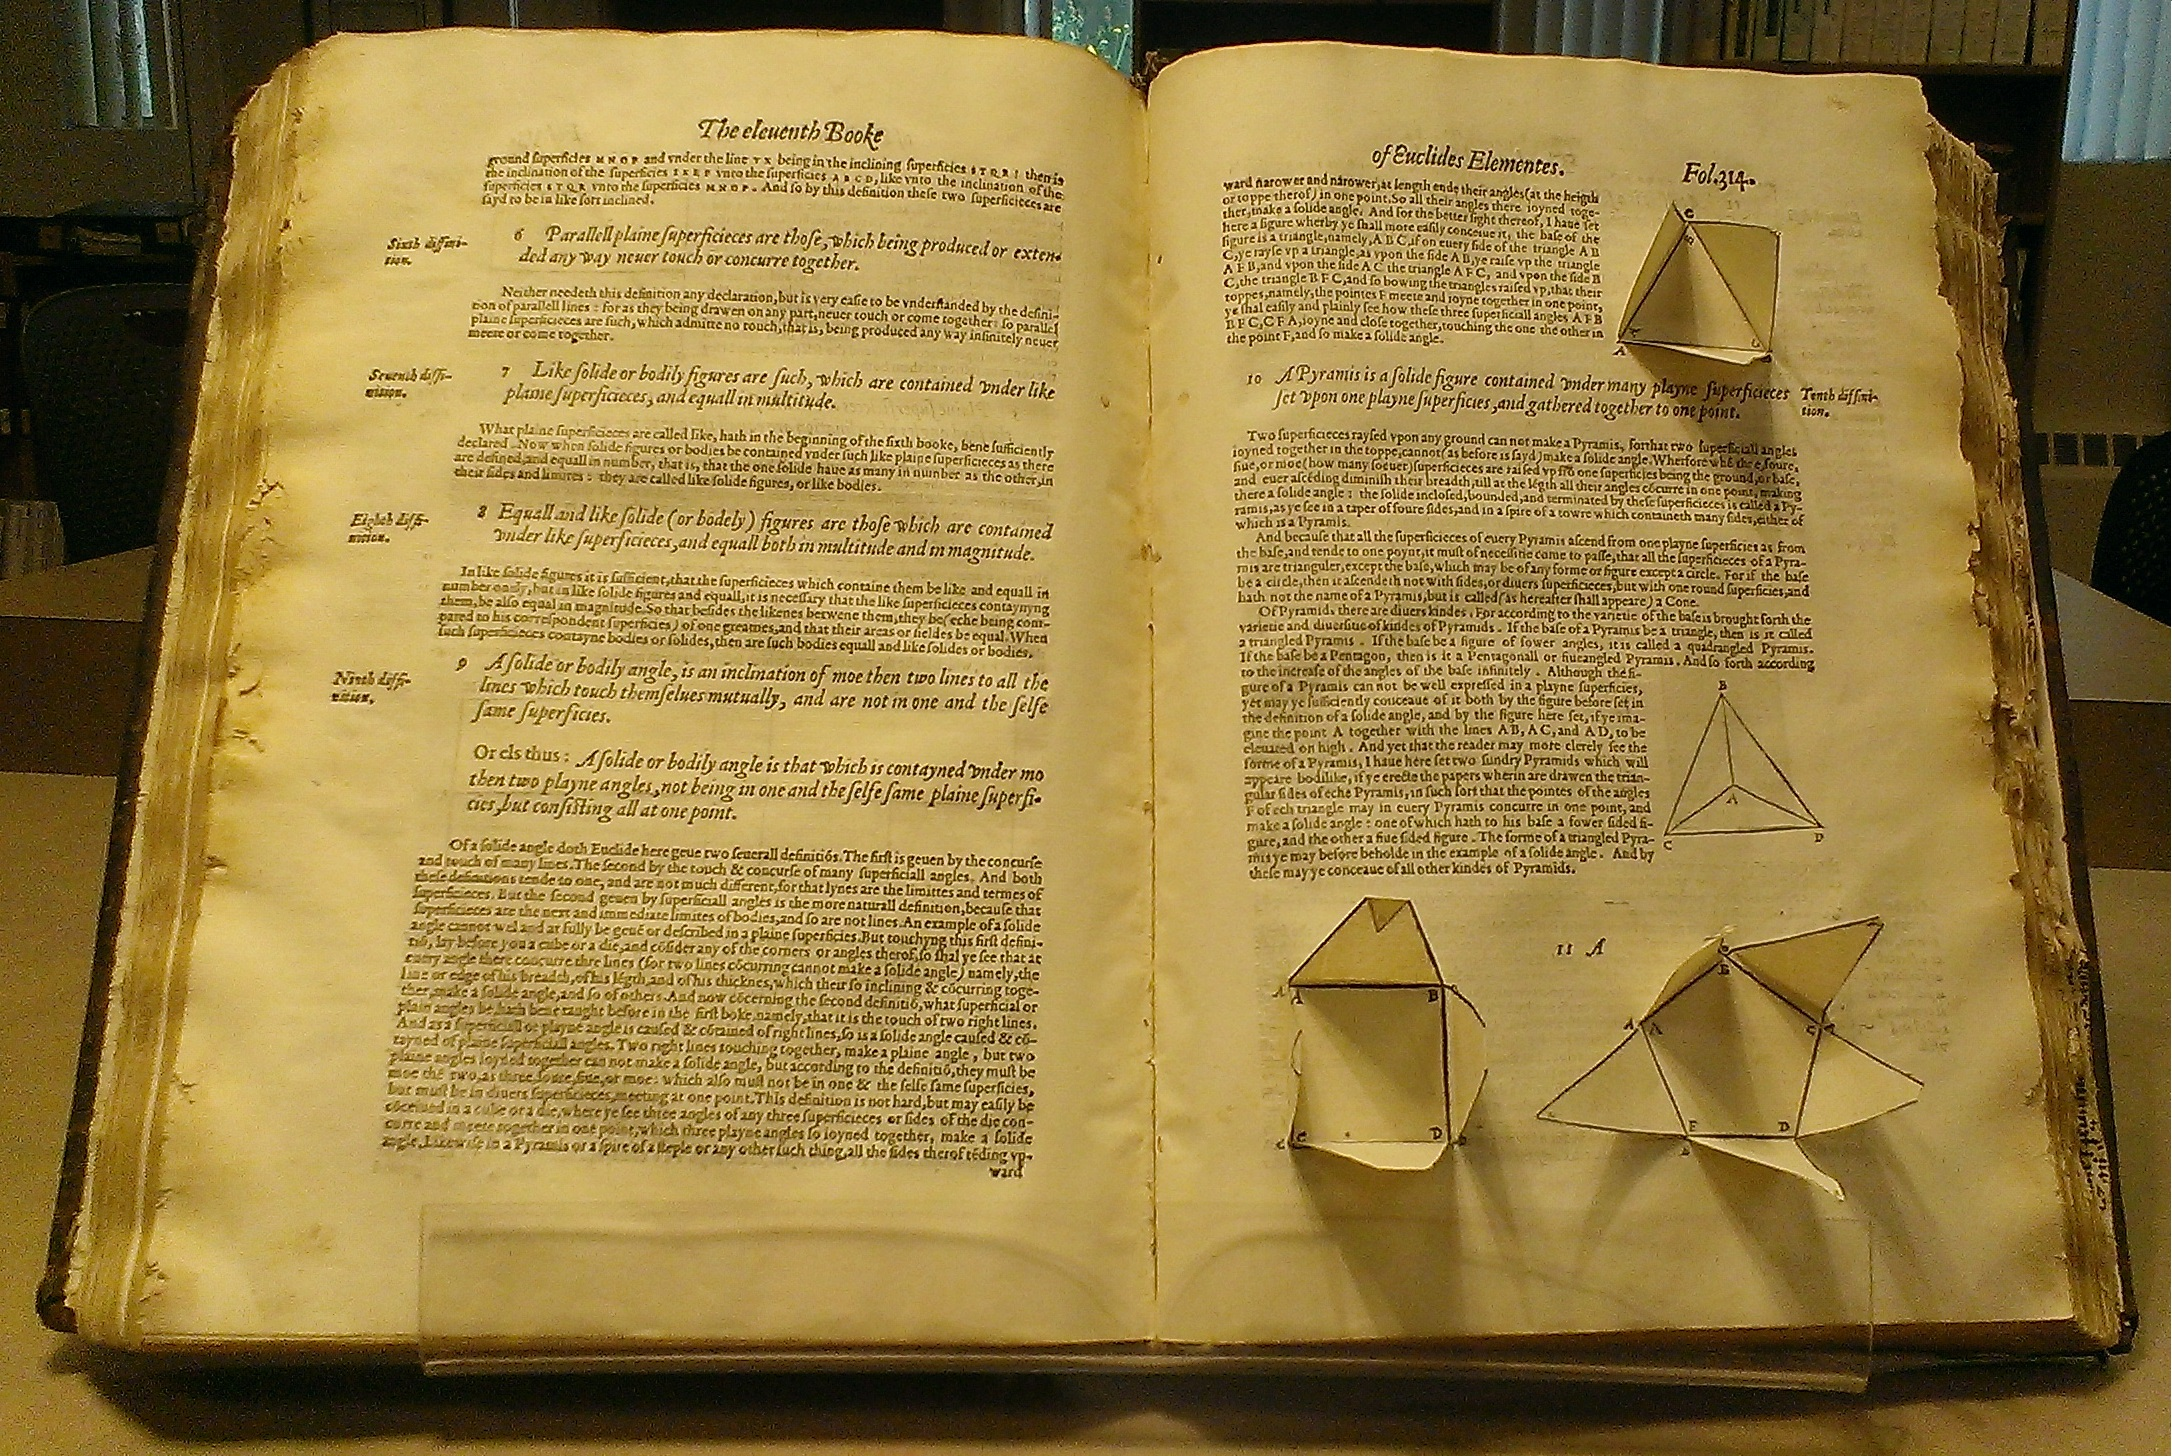
\includegraphics[width=0.95\linewidth]{euclid3}\\
		Pop-up edition, 1500s
	\end{minipage}%
	\begin{minipage}[b]{0.33\linewidth}\vspace{0pt}
		\centering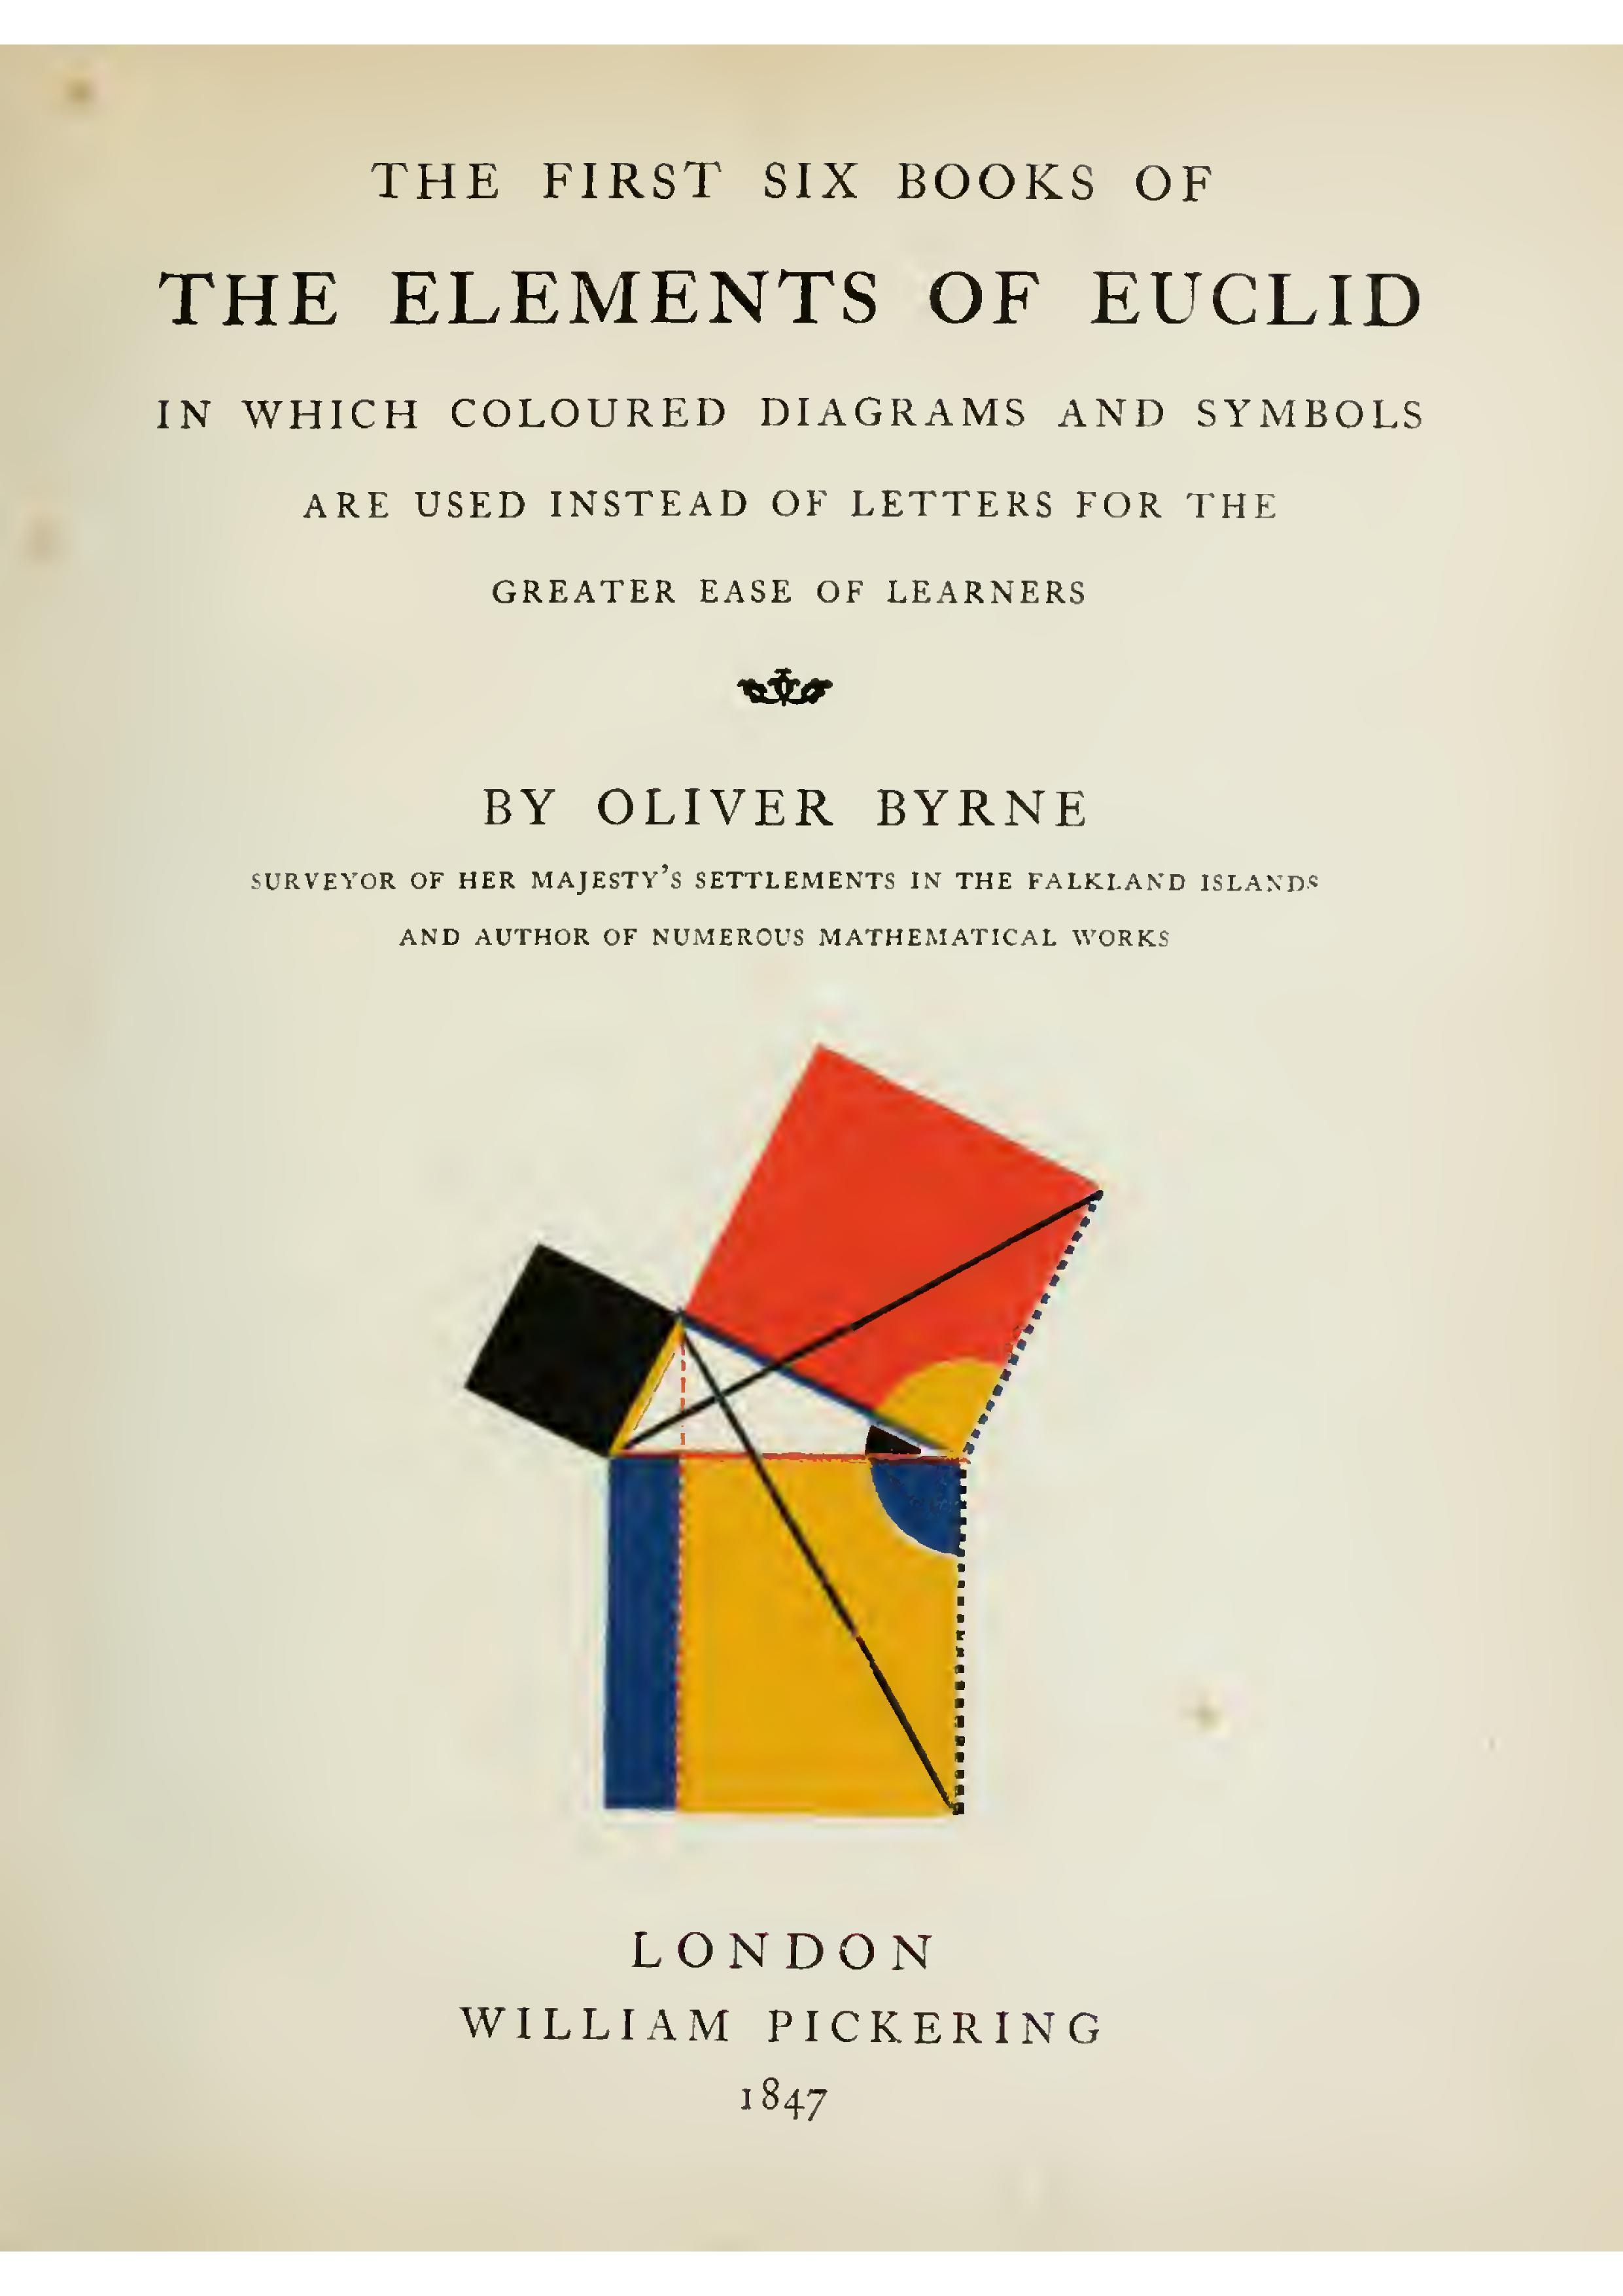
\includegraphics[width=0.95\linewidth]{euclid5}\\
		Color edition, 1847
	\end{minipage}
\end{center}

You can download Byrne's color edition \href{http://math.uci.edu/~ndonalds/Elements-I-VI.pdf}{here} (very large file!). It is notably different from many earlier editions: it contains a much longer list of definitions, inserts many more axioms, and relabels propositions 4 and 5 as axioms (pages xviii--xxiii). The picture on the cover page is Euclid's proof of Pythagoras' Theorem (Book I, Thm.\ 47).
\goodbreak


\boldsubsubsection{A Brief Overview of the \emph{Elements}}

The \emph{Elements} consists of thirteen books covering two- and three-dimensional geometry, computations and number theory. Whether some version of every book was written by Euclid himself is unknown.\footnote{It is not even certain that Euclid was a single person as opposed to a figurehead or a name for a collective. It is hardly surprising that we know so little about someone who lived 2300 years ago. The same questions are sometimes raised about William Shakespeare who lived only 400 years ago!} The key feature of the \emph{Elements} is its \emph{axiomatic} presentation. Each book begins with a list of axioms/postulates and definitions and proceeds to prove theorems deduced from these. This \emph{axiomatic method} is essentially universal in modern mathematics, and its advent is fundamentally what sets Greek mathematics apart from everything that came before.\smallbreak

We briefly discuss Book I, then give some flavor of the remainder of the text with a few example results. Several examples of material from later books were mentioned in the previous section.


\boldinline{Book I}

Consists of 48 theorems, culminating with Pythagoras' and its converse. It seems likely that Euclid organized Book I with the goal of proving this important result in a rigorous manner: recall (pg.\,\pageref{pthagorig}) how the Pythagorean `proof' relied on the erroneous notion of commensurability. Here are the postulates from Book I: the first three are what define ruler-and-compass constructions (pg.\,\pageref{pg:construction}).

\begin{itemize}\itemsep0pt
  \item[P1] Given any two points, a straight line can be drawn between them
  \item[P2] Any line may be indefinitely extended
  \item[P3] Given a center and a radius, a circle may be drawn
  \item[P4] All right angles are equal to each other
  \item[P5] If a straight line crosses two others so that the angles on the same side make less than two right angles, then the two lines meet on that side of the original.
\end{itemize}

The fifth postulate is awkwardly phrased. An equivalent modern statement is \emph{Playfair's axiom}:
\begin{quote}
	There is at most one parallel through a given point not on line.
\end{quote}
For centuries, mathematicians tried to prove that this postulate was a theorem of the others until; it was eventually shown to be necessary with the advent of hyperbolic geometry in the 1800s. Euclid's refusal to use the parallel postulate until Theorem 29 suggests he understood this awkwardness.\smallbreak


Theorems are generally presented as \emph{problems}: a pictorial construction is provided, then Euclid proves that the construction really solves the problem. Here is Euclid's first theorem.

\begin{thm*}{I.\,1}{}\phantomsection\label{pg:euclidI1}
	Problem: To construct an equilateral triangle on a given segment.
\end{thm*}

\begin{proof}
	Given 
\includegraphics{euclid-I1a} construct two circles (P3)\quad\raisebox{-16pt}{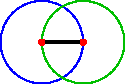
\includegraphics{euclid-I1b}}\par\vspace{-23pt}
	Join one of the circle intersections to the endpoints of the original segment (P1)\quad \raisebox{-28pt}{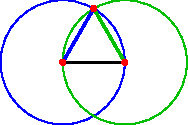
\includegraphics{euclid-I1c}}\par\vspace{-11pt}
	The result is an equilateral triangle; indeed the three sides are congruent, for\par \raisebox{-10pt}{
\includegraphics{euclid-I1d}} are radii of a common circle,
	as are \raisebox{-10pt}{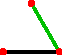
\includegraphics{euclid-I1e}}
\end{proof}

\goodbreak

After this Euclid proceeds to establish several well-known results. Since this isn't a geometry class, we'll omit most of the details. You can find more of these \href{http://math.uci.edu/~ndonalds/math161/euclid.pdf}{here,} in \href{http://math.uci.edu/~ndonalds/Elements-I-VI.pdf}{Byrne,} or elsewhere.

\begin{description}
  \item[\normalfont Thm\ I.\,4] Side angle side: if triangles have two pairs of congruent sides and the angles between them are also congruent, then the remaining sides and angles are congruent.
  \item[\normalfont Thm\ I.\,15] Vertical angles: if two lines meet, then the opposite angles made are congruent.
  \item[\normalfont Thms\ I.\,27 \& 29] Angles and parallels: if a line falls on two other lines, then the two lines are parallel if and only if the alternate angles are congruent ($\alpha\cong \beta$ in the picture).
  \begin{center}
	  \begin{tabular}{@{}c@{\qquad}c@{\quad}c@{\quad}c@{}}
		  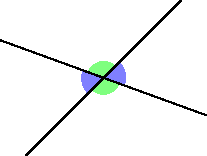
\includegraphics{euclid-I15}
		  &
		  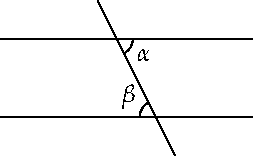
\includegraphics{euclid-I29}
		  &
		  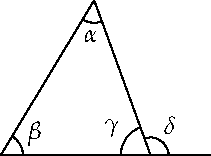
\includegraphics{euclid-I32}
		  &
		  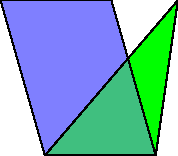
\includegraphics{euclid-I41}
		  \\
		  Thm I.\,15
		  &
		  Thms I.\,27/29
		  &
		  Thm I.\,32
		  &
		  Thm I.\,41
	  \end{tabular}
  \end{center}
  \item[\normalfont Thm\ I.\,32] Angle sums in a triangle: if one side of a triangle is protruded, the exterior angle equals the sum of the opposite interior angles.\par
  In the picture $\alpha+\beta=\delta$; in modern language $\alpha+\beta+\gamma=\ang{180}$.
  \item[\normalfont Thm\ I.\,41] A parallelogram and triangle on the same base and with the same height have area in the ratio 2:1.
\end{description}

The last two results of Book I are Pythagoras and its converse.

\begin{thm*}{I.\,47}{}
	The square on the hypotenuse of a right-triangle has area equal to the sum of the areas of the squares on the remaining sides.
\end{thm*}

\begin{proof}
	Given a right-angle at $A$, drop the perpendicular from $A$ across $\nm{BC}$ to $L$.\par
	\begin{minipage}[t]{0.6\linewidth}\vspace{-5pt}
		$\triangle FBC$ and $\square ABFG$ share the same base $\cl{BF}$ and height $\cl{AB}$. By Thm I.\,41,
		\[
			\operatorname{area}(\square ABFG)=2\operatorname{area}(\triangle BCF)
		\]
		Similarly (base $\cl{BD}$, height $\cl{BO}$)
		\[
			\operatorname{area}(\square BOLD)=2\operatorname{area}(\triangle ABD)
		\]
		Side-Angle-Side (Thm I.\,4) $\implies\triangle ABD\cong\triangle FBC$; the triangles have the same area, and so
		\[
			\operatorname{area}(\textcolor{red}{\square ABFG})=\operatorname{area}(\textcolor{red}{\square BOLD})
		\]
		Similarly $\operatorname{area}(\textcolor{Green}{\square ACKH})=\operatorname{area}(\textcolor{Green}{\square OCEL})$.
	\end{minipage}
	\hfill
	\begin{minipage}[t]{0.39\linewidth}\vspace{-12pt}
		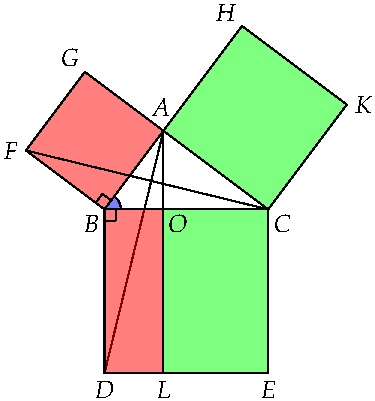
\includegraphics{euclid-I47}
	\end{minipage}
\end{proof}

The converse (Thm I.\,48) is Exercise \ref{exs:pythagconv}.


\goodbreak%\clearpage


\begin{description}
	\item[Book II]\lstsp Geometric solutions to problems that would now be treated using algebra. Much of this is attributable to the Pythagoreans.\par
	(Thm II.\,11)\lstsp A segment may be divided so that the rectangle contained by the whole and one of the sub-segments is equal to the square on the remaining sub-segment.\par
	We rephrase this in modern language. Suppose the given segment $\cl{AB}$ has length $a$, our goal is to find $H$ on $\cl{AB}$ such that $\nm{AH}=x$ and $\textcolor{Green}{x^2}=\textcolor{blue}{a(a-x)}$. Euclid is providing a \emph{geometric solution} to a quadratic equation!\par
	\begin{minipage}[t]{0.69\linewidth}\vspace{-8pt}
		\begin{enumerate}\itemsep2pt
		  \item Construct $\square ABDC$ on $\cl{AB}$
			\item Let $E$ be the midpoint of $\cl{AC}$ and connect $\cl{EB}$
			\item Extend $\cl{AC}$ and lay off $\cl{EF}\cong\cl{EB}$ on $\cl{AC}$ extended
			\item Construct $\square AFGH$ and drop the perpendicular to $I$
			\item To finish: prove that $\operatorname{area}(\textcolor{Green}{\square AFGH}) =\operatorname{area}(\textcolor{blue}{\square BDIH})$
		\end{enumerate}
		The solution $x=\nm{AH}=\frac{\sqrt 5-1}2a$ \, means that $\cl{AH}:\cl{HB}$ is the \emph{golden ratio.}
	\end{minipage}
	\hfill
	\begin{minipage}[t]{0.3\linewidth}\vspace{-10pt}
		\flushright
		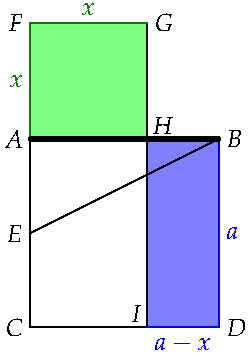
\includegraphics[scale=0.95]{euclid-II11}
	\end{minipage}
	\medbreak



	\begin{minipage}[t]{0.74\linewidth}\vspace{0pt}
		\item[Book III]\lstsp Theorems regarding circles and tangency. Most of this material likely came from Hippocrates.\phantomsection\label{pg:thalesthm}\par
		  (Thm III.\,31)\lstsp Thales' Thm: a triangle in a semi-circle is right-angled.  
	\end{minipage}
	\hfill
	\begin{minipage}[t]{0.25\linewidth}\vspace{0pt}
		\flushright
		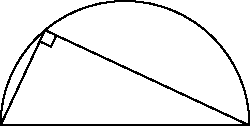
\includegraphics[scale=0.9]{euclid-III31}
	\end{minipage}


	\item[Book IV]\lstsp Construction of regular 3, 4, 5, 6 and 15-sided polygons inscribing and exscribing a circle. Also likely the work of Hippocrates.
	
	\item[Book V]\lstsp Ratios and magnitudes à la Eudoxus.\par
		(Thm V.\,11)\lstsp If $a:b=c:d$ and $c:d=e:f$ then $a:b=e:f$
	
	
	\item[Book VI]\lstsp Ratios of magnitudes applied to geometry (similarity results).\smallbreak
	  (Thm VI.\,4)\lstsp Triangles with equal angles have corresponding sides proportional.\smallbreak
	  (Thm VI.\,8)\lstsp The altitude from the right angle of a right triangle divides it into two triangles similar to each other and the the original.\par
	  (Thm VI.\,31)\lstsp Corrected Pythagorean proof (pg.\,\pageref{pthagorig}) of Pythagoras' using Eudoxus' proportions and Thm VI.\,8.
	  
	
	\item[Book VII]\lstsp Divisibility and the Euclidean algorithm. Probably due to the Pythagoreans and Theaetetus.
	
	
	\item[Book VIII]\lstsp Number progressions, geometric sequences. Possibly due to studies in music by Archytas (a Pythagorean who taught Plato mathematics).
	
	
	\item[Book IX]\lstsp Number Theory: even/odd + perfect numbers.\par
	(Thm IX.\,20)\lstsp There are infinitely many primes.
	
	
	\item[Book X]\lstsp Discussion of commensurable and incommensurable ratios. Long and difficult, possibly derived from Theaetetus.
	
	
	\item[Book XI]\lstsp Solid geometry (lines/planes in 3D).\par
		(Thm XI.\,28)\lstsp A parallelepiped is bisected by its diagonal plane.
		
		
	\item[Book XII]\lstsp Ratios of areas and volumes (Eudoxus).\par
		(Thm XII.\,2) The areas of circles are in the same ratio as the squares on their diameters.
	
	
	\item[Book XIII]\lstsp Construction of regular polyhedra inside a sphere and their classification.\par
		(Thm XIII.\,10)\lstsp If a regular pentagon, hexagon and decagon are inscribed in the same circle, then their sides form a right-triangle.
\end{description}

One could study the \emph{Elements} and its influence for a lifetime and not be done! Hopefully this very brief overview convinces you why the book had such a profound impact on mathematics.


\begin{exercises}
	\exstart Prove Thales' Theorem (III.\,31) (pg.\,\pageref{pg:thalesthm}).\vspace{-5pt}
	
	\begin{enumerate}\setcounter{enumi}{1}
	  \item[](\emph{Hint: start by joining the center of the circle to the apex of the triangle\ldots})
	  
	  \begin{minipage}[t]{0.7\linewidth}\vspace{0pt}
		  \item%[3-6]
		  %   Prove Thm I.\,32: the sum of the three interior angles of a triangle is equal to two right angles. Show that the proof depends on Thm I.\,29, and therefore on the parallel postulate.
		  Use the picture to provide a proof of Thm I.\,32: the sum of the three interior angles of a triangle is equal to two right angles.\par
		  Show that the proof depends on Thm I.\,29, and therefore on the parallel postulate.\par
		  (\emph{This isn't quite the same as Euclid's argument})
	  \end{minipage}
	  \hfill
	  \begin{minipage}[t]{0.29\linewidth}\vspace{0pt}
	  	\flushright
	  	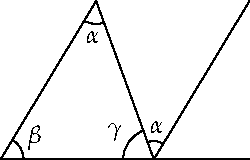
\includegraphics{euclid-I32proof}
	  \end{minipage}
	  
	  \begin{minipage}[t]{0.7\linewidth}\vspace{0pt}
		  \item\label{exs:pythagconv} Suppose that the square on side $\cl{BC}$ of $\triangle ABC$ has the same area as the sum of the squares on the other sides $\cl{AB}$, $\cl{AC}$. As in the picture, draw a perpendicular $\cl{AD}\cong \cl{AB}$.
		  \begin{enumerate}
		    \item Explain why $\cl{DC}\cong\cl{BC}$.
		    \item Hence conclude that $\triangle ABC$ is right-angled at $A$.
		  \end{enumerate}
	  \end{minipage}
	  \hfill
	  \begin{minipage}[t]{0.29\linewidth}\vspace{0pt}
	  	\flushright
	  	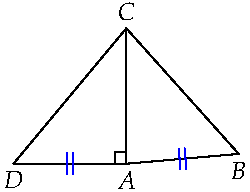
\includegraphics{euclid-I48}
	  \end{minipage}
	
	
	  \item%[3-12]
	  Prove Thm III.\,3:\lstsp A diameter of a circle bisects a chord if and only if it is perpendicular to the chord.
	  
	  
	  \item Verify that Euclid's construction for Thm II.\,11 really does solve the given problem.\par
	  (\emph{You can use modern algebra!})
	  
	    
	  \item%[3-28]
	  Draw a semi-circle with diameter $9+5=14$. Solve the equation $\frac 9x=\frac x5$ \emph{geometrically,} by constructing a vertical line whose length is $x$.
	  
	  
	  
	  \item%[2-14]
	  Show that areas of similar segments of circles are proportional to the squares of the length of their chords.\par
	  (\emph{You may assume that areas of circles are proportional to the squares on their diameters and can use modern algebra/trigonometry if you wish})
	\end{enumerate}

\end{exercises}

\clearpage


\subsection{Archimedes of Syracuse}\label{sec:archimedes}

Archimedes (287--212\BC) is arguably the greatest ancient mathematician. Syracuse is on the island of Sicily at the foot of the Italian peninsula; at the time of Archimedes' birth this was a Greek city-state, though under threat from the expanding Roman Empire. Archimedes famously helped defend Syracuse against the Romans using catapults, though he ultimately died at their hands after the city fell. He is believed to have travelled to Alexandria in his youth and perhaps studied with scholars at the library, including Eratosthenes (pg.\,\pageref{pg:eratosthenes}).\smallbreak

Archimedes' genius was practical not just mathematical. Beyond his anti-Roman catapults, he is credited with a large number of inventions and technical innovations, including \href{https://en.wikipedia.org/wiki/Archimedes'_screw}{\emph{Archimedes' screw,}} still used in modern irrigation systems to elevate water. He is acknowledged as the founder of \emph{hydrostatics,} where \emph{Archimedes' principle} states that an object immersed in water loses weight equal to that of the displaced water. A famous story recounts Archimedes using this to detect whether a smith had used all the gold he had been given in the manufacture of a crown.\smallbreak

\begin{minipage}[t]{0.69\linewidth}\vspace{0pt}
	\boldinline{Example}
	A cube with side length 20\,cm floats such that the water-line is halfway up the cube. By Archimedes' principle, the weight of the cube is the same as that of the volume of displaced water:
	\[
		20\times 20\times 10=4000\,\text{cm}^3
	\]
	which has a weight (mass) of roughly 4\,kg.
\end{minipage}
\hfill
\begin{minipage}[t]{0.3\linewidth}\vspace{0pt}
	\flushright
	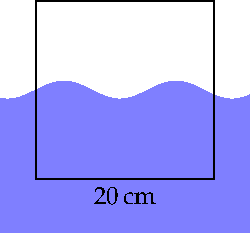
\includegraphics{archimedes-cube}
\end{minipage}



\boldinline{Levers}

Archimedes made great study of levers, both for practical purposes and as a method of calculation.

\begin{center}
	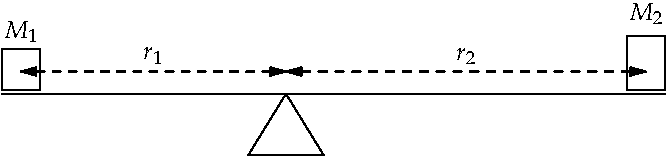
\includegraphics{archimedes-lever}
\end{center}

Given masses $M_1$, $M_2$ located distances $r_1$, $r_2$ from a pivot, Archimedes states:
\begin{itemize}%\itemsep0pt
  \item The lever balances $\iff M_1:M_2=r_2:r_1$
  \item The lever rotates clockwise $\iff M_1:M_2<r_2:r_1$
  \item The lever rotates counter-clockwise $\iff M_1:M_2>r_2:r_1$
\end{itemize}
In modern terms we'd compare the \emph{torques} $\tau_1=M_1r_1$ and $\tau_2=M_2r_2$. Since torque requires the multiplication of non-numerical quantities, Archimedes would instead have considered this using Eudoxus' theory of proportions.\par
For example, to find the mass $M_2$ required to balance a lever given $M_1=12$\,lb, $r_1=4$\,ft and $r_2=3$\,ft, Archimedes would have observed that
\[
	M_2:M_1=4:3\implies M_2=16\,\text{lb}
\]
\goodbreak


\boldinline{\emph{The Method}: is Archimedes the founder of calculus?}

A previously unknown work of Archimedes was discovered in 1899. As an amazing application of the lever principle, Archimedes makes an argument that looks remarkably like modern calculus; he could be claimed to be its earliest practitioner by 1800 years! The method was outlined in a letter to Eratosthenes and includes part of an argument for proving Archimedes' favorite theorem, a picture of this result was engraved on his tomb.

\begin{thm*}{}{}
	A cone, hemisphere and cylinder with the same base and height have volumes in the ratio $1:2:3$. Using modern formulæ, if the height is $r$, then the volumes are $\frac 13\pi r^3:\frac 23\pi r^3:\pi r^3$.
\end{thm*}
\phantomsection\label{pg:archmethod}

\begin{minipage}[t]{0.67\linewidth}\vspace{-3pt}
	Here is a modernized version of half the result. Suppose the `base' is a disk with radius 1. Archimedes removes the hemisphere from the cylinder and places the cone beneath. Compare the \textcolor{red}{cross-sections} the same distance $y$ from the apex of the cone.
	\begin{itemize}\itemsep0pt
	  \item The circular cross-section of the cone has radius $y$ whence its area is proportional to the square on the radius: $\pi y^2$.
		\item The upper annular cross-section has area proportional to the difference of the squares on the radius of the cylinder and on the distance $x$. By Pythagoras' the cross-sectional area is
		\[
			\pi(1^2-x^2)=\pi(1-(1-y^2))=\pi y^2
		\]
	\end{itemize}
\end{minipage}
\hfill
\begin{minipage}[t]{0.32\linewidth}\vspace{-3pt}
	\flushright
	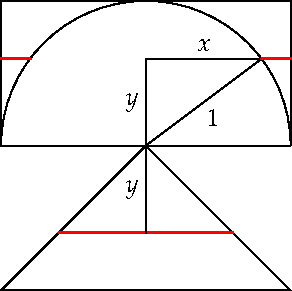
\includegraphics{archimedes-spherecone}
\end{minipage}
\bigbreak
The cross-sections are therefore in balance with respect to a vertical lever whose pivot lies at the center of the picture. Archimedes concludes that the cone and the upper-figure are in balance: that is
\[
	V_\text{cone}=V_\text{cylinder}-V_\text{hemisphere}
\]
in line with the desired ratios.
\bigbreak


Here is another argument of Archimedes' with a suggestion of calculus. A disk comprises infinitely many concentric circles, the circumference of each being proportional to its radius. `Unwind' these circles to obtain a triangle; one side is the radius of the disk, the other its circumference. The area of a circle is therefore that of a triangle with sides the radius and circumference of the circle: $A=\frac 12rc$.
\begin{center}
	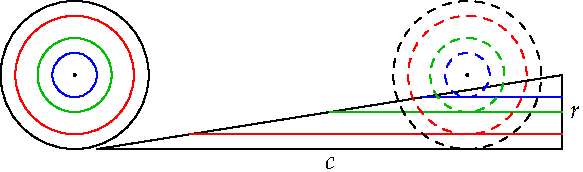
\includegraphics{archimedes-circle}
\end{center}

\emph{The Method} includes several of these calculus-like discussions. While efficient, Archimedes felt that his approach didn't constitute a proof and provided alternative arguments elsewhere in his writings. The essential problem is this;
\begin{quote}
  Can we really say that an area \emph{equals} its cross-sectional lines? Or that a volume \emph{equals} its cross-sectional areas? Lines have no width so if we add them up we have no area. If they have width, then infinitely many of them have infinite area.
\end{quote}
These are really variations of Zeno's paradoxes (pg.\,\pageref{pg:zeno}) regarding infinitesimals and indivisibles!
\goodbreak

Archimedes' arguments would be resurrected in the early 1600s by Cavalieri and Galileo as the development of calculus gathered pace. The same duality of presentation characterised this later development: Newton and others found the infinitesimal approach efficient, but felt the need to present \emph{geometric} proofs to convince readers that their results weren't mere trickery.\smallbreak
It is tempting to imagine what might have happened if Archimedes' \emph{method} had been accepted and preserved as part of the Greek canon; if calculus had been developed 1800 years earlier, how might this have affected technological development? Would the space-race have happened in \AD 500?! %It is a romantic notion certainly, but also a simplistic one. There were other factors at play in the 1600s that made the development of calculus more likely. Still, history is full of fun \emph{what-if}'s to ponder\ldots\par


\boldinline{Quadratures} Archimedes also approximated areas and arc-lengths of various figures using limit-like argumentation. Here is how he approached the area/circumference of a circle.\phantomsection\label{pg:archquadcircle}

\begin{enumerate}\itemsep0pt
  \item Inscribe a regular hexagon in a circle (of radius 1 say) and compute its perimeter ($6$).
  \item Halve each angle to obtain a regular dodecagon: compute its perimeter ($12\sqrt{2-\sqrt 3}$).
  \item Repeat the angle-halving process: Archimedes did this with 24-, 48- and 96-gons to obtain an increasing sequence of perimeters bounded above by the circumference of the circle ($2\pi$).
  \item Repeat the same calculation with circumscribed polygons to obtain a decreasing sequence of over-estimates.
  \item Using 96-sided polygons allowed Archimedes to obtain the estimate $3\frac{10}{71}<\pi<3\frac 17$.
\end{enumerate}

\begin{minipage}[t]{0.64\linewidth}\vspace{-5pt}
	Archimedes' halving process relied on an induction step, an approximation of which we mimic here. Suppose we have an isosceles triangle with equal legs 1, altitude $\textcolor{blue}{d_n}$, and chord $2\textcolor{red}{h_n}$. We halve the angle to find the new altitude $\textcolor{Green}{d_{n+1}}$ and chord $2\textcolor{orange}{h_{n+1}}$. Everything follows from three applications of Pythagoras':
	\begin{gather*}
		1=\textcolor{blue}{d}^2_{\textcolor{blue}{n}} +\textcolor{red}{h}^2_{\textcolor{red}{n}}\\
		(2\textcolor{orange}{h_{n+1}})^2=\textcolor{red}{h_n}\!\!\!\!\!{\phantom{h}}^2 +(\textcolor{Brown}{1-d_n})^2\\ 
		1=\textcolor{Green}{d}^2_{\textcolor{Green}{n+1}} +\textcolor{orange}{h}^2_{\textcolor{orange}{n+1}}
	\end{gather*}
	Expanding and cancelling, we obtain
	\[
		\textcolor{Green}{d}^2_{\textcolor{Green}{n+1}} =\frac 12(1+\textcolor{blue}{d}_{\textcolor{blue}{n}}),\qquad \textcolor{orange}{h}^2_{\textcolor{orange}{n+1}} =1-\textcolor{Green}{d}^2_{\textcolor{Green}{n+1}} =\frac 12(1-\textcolor{blue}{d}_{\textcolor{blue}{n}})
	\]
\end{minipage}
\hfill
\begin{minipage}[t]{0.35\linewidth}\vspace{0pt}
	\flushright
	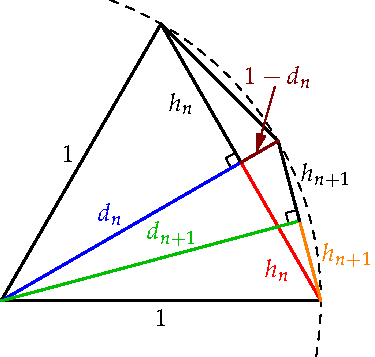
\includegraphics[scale=0.9]{archimedes-hex}
\end{minipage}
\medbreak
Since $d_0=\frac{\sqrt 3}2$ and $h_0=\frac 12$, we may compute the entirety of both sequences:
\begin{gather*}
	d_1=\frac 12\sqrt{2+\sqrt 3},\quad d_2=\frac 12\sqrt{2+\sqrt{2+\sqrt 3}},\quad\ldots\quad d_n=\frac 12\sqrt{2+\sqrt{2+\cdots+\sqrt{2+\sqrt 3}}}\\
	h_1=\frac 12\sqrt{2-\sqrt 3},\quad h_2=\frac 12\sqrt{2-\sqrt{2+\sqrt 3}},\quad\ldots\quad h_n=\frac 12\sqrt{2-\sqrt{2+\cdots+\sqrt{2+\sqrt 3}}}
\end{gather*}
where the $n\th$ terms have $n$ copies of the digit 2 under the square-root. The circumference and area of the $6\cdot 2^n$-sided polygon inscribed in the circle are therefore
\[
	C_n=12\cdot 2^nh_n,\qquad A_n=6\cdot 2^nd_nh_n=6\cdot 2^{n-1}h_{n-1}=\frac 12C_{n-1}
\]
These sequences increase to $2\pi$ and $\pi$ respectively. For a 96-sided polygon, Archimedes would have had to approximate
\[
	C_4=12\cdot 2^4h_4=96\sqrt{2-\sqrt{2+\sqrt{2+\sqrt{2+\sqrt 3}}}}> 6.282\implies \pi>3.141>3\frac{10}{71}
\]




\boldsubsubsection{Other Highlights of the later Greek Period: 300\BC--\AD 500}\phantomsection\label{pg:eratosthenes}

We'll consider ancient astronomy, including Greek contributions, in the next chapter. Here are a few of the other developments of the late Greek period and some historical context.

\begin{itemize}\itemsep1pt
  \item Eratosthenes (276--194\BC) grew up in Cyrene (c.\,500 miles west of Alexandria in modern-day Libya) and moved to Alexandria in adulthood to become its librarian. He is credited with a simple algorithm for finding primes: the \emph{Sieve of Eratosthenes.}
  \begin{itemize}
    \item List the integers $n\ge 2$.
    \item Leave 2 and delete all its multiples.
    \item Leave 3 and delete its multiples.
    \item Repeat ad infinitum: each time one reaches a number, leave it and delete its multiples.
    \item The remaining list contains all the primes. 
  \end{itemize}

  \item Apollonius (225\BC) writes an eight-volume book on conic sections building on earlier work of Menaechmusus (350\BC).
  
  \item By 146\BC{} the Greek empire had fallen under Roman rule. Alexandria remained important. Educated Greeks still spoke and wrote in Greek rather than (Roman) Latin. For context, Julius Caesar ruled Rome around this time (died 44\BC).
  %\item Hipparchus (140\BC) computed chords (essentially sine tables, although the word was not used) for Astronomical purposes.
  
  \item Heron (\AD 75) proves the formula $\sqrt{s(s-a)(s-b)(s-c)}$ for the area of triangle, where $s=\frac 12(a+b+c)$ is the semi-perimeter. This was likely known to Archimedes; Heron's work was a compilation of earlier mathematics.
  
  \item Around \AD 100 the Neopythagorean's worked in Alexandria, studying music, philosophy, and number, with the intent of reviving the teachings of Pythagoras.
  %\item Ptolemy (\AD 150) extended the work of Hipparchus on trigonometry and wrote the astronomical masterwork \emph{Almagest.} We shall study this in the next section.
  
  \item Around \AD 400, Theon and Hypatia produce the most widely-read edition of Euclid's \emph{Elements} as well as improving upon several earlier mathematical topics.
  
  \item In \AD 395 the Roman empire split into eastern and western parts centered on Rome and Byzantium/Constantinople. The western empire rapidly declined under the pressures of corruption and barbarian attacks, collapsing completely by \AD 500. Alexandria experienced riots and a bloody power-struggle (Hypatia was murdered by a mob in 415) and the library of Alexandria was severely damaged and possibly destroyed at this time. In 642, Alexandria was captured by the new Islamic caliphate. Much of the material in the library survived by being copied and transported to various places of learning; particularly Constantinople and Baghdad. For the next 600 years, the knowledge of Alexandria was largely a mystery to (western) Europe.
\end{itemize}


\goodbreak


\begin{exercises}
	\exstart %[4-2]
	If a weight of 8\,kg is placed 10\,m from the pivot of a lever and a weight of 12\,kg is placed 8\,m from the pivot in the opposite direction, toward which weight will the lever incline? Answer using Archimedes' language.
	
	
	\begin{enumerate}\setcounter{enumi}{1}
	  \item Use Eratosthenes' Sieve to find all the primes $<100$.
	  
	  
	  \item\begin{enumerate}
	    \item Prove Heron's formula as follows.
		 	\begin{enumerate}
			 	\begin{minipage}[t]{0.68\linewidth}\vspace{-5pt}
			    \item Let $h$ be the altitude and $x$ the base of the left-hand right-triangle. Apply Pythagoras' to the two right-triangles to show that
			    \[
			    	x=\frac{a^2+b^2-c^2}{2a}
			    \]
			 	\end{minipage}
			 	\hfill
			 	\begin{minipage}[t]{0.31\linewidth}\vspace{-15pt}
			 		\flushright
			 		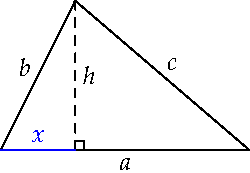
\includegraphics{archimedes-heron}
			 	\end{minipage}
			  \item Substitute in $h^2=b^2-x^2$ to find $h$ in terms of $a,b,c$ and thus deduce Heron's formula.
		  \end{enumerate}
	  
	  	\item Find the area of a triangle with sides 4, 7 and 10.
	  \end{enumerate}
	
	  
	  \item Suppose $C_n$ is the circumference of a $6\cdot 2^n$-sided inscribed polygon in a unit circle. Show that the circumference of the corresponding \emph{circumscribed} polygon is $C^{\text{ex}}_n=\frac 1{d_n}C_n$.
	  
	  \item Use the modern formula $A=\frac 12ab\sin C$ to prove that, for any $k\in\N$
	  \[
	  	\frac 12k\sin\frac{2\pi}k<\pi<k\tan\frac\pi k
	  \]
	  Moreover, explain why both sides converge to $\pi$.
	  
	  \item%[4-4]
	  Instead of modern algebra, Archimedes used several geometric lemmas to help find the areas of polygons inscribed in and circumscribing circles. Here is one; prove it!\par
	  Let $\cl{OA}$ be the radius of a circle and $\cl{AC}$ be tangent to the circle at $A$. Let $D$ lie on $\cl{AC}$ such that $\cl{OD}$ bisects $\angle COA$. Then
	  \[
	  	\frac{\nm{DA}}{\nm{OA}}=\frac{\nm{CA}}{\nm{CO}+\nm{OA}}\quad\text{and}\quad \nm{DO}^2=\nm{OA}^2+\nm{DA}^2
	  \]
	  (\emph{Hint: draw a picture and let $T$ be the intersection of the circle and $\cl{OC}$})
	 % If you want a challenge, try proving the second lemma mentioned in the book\ldots
	 
	 	\item (Hard)\lstsp Archimedes used a geometric series approach to evaluate the area inside a parabola. Use modern algebra for this question.\par
	 	\begin{minipage}[t]{0.6\linewidth}\vspace{-5pt}
	 	 	\begin{enumerate}
	  		\item Suppose $y=a+bx+cx^2$ is the equation of a \textcolor{blue}{parabola}. If $P,Q,R$ have $x$ co-ordinates in an arithmetic sequence $x-\epsilon,x,x+\epsilon$, show that the area of $\triangle PQR$ is $A=\nm c\!\epsilon^3$; \emph{independent of $x$}!
	  		\item With reference to the picture, if $A$ is the area of the \textcolor{Green}{large triangle}, explain why the smaller triangle has area $A_1=\frac 18A$.
	  		\item Use a geometric series to prove that the area inside the parabola bounded by $\cl{PR}$ is $\frac 43A$
	 		\end{enumerate}
	 	\end{minipage}
	 	\hfill
	 	\begin{minipage}[t]{0.39\linewidth}\vspace{-5pt}
	 		\flushright
	 		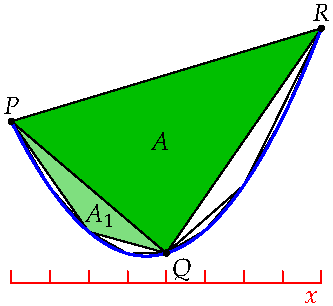
\includegraphics{archimedes-parabola}
	 	\end{minipage}
	
	\end{enumerate}
\end{exercises}






% \subsubsection*{Conic Sections}
% 
% Menaechmusus (350BC): defined conic sections. Started with a single cone and define
% 
% Parabola: slice right-angled cone perpendicular to generator\\
% Hyperbola: slice obtuse-angled cone perp to generator\\
% Ellipse: slice acute-angled cone perp to generator
% 
% 
% Used double-cone of any size and cut by any plane: decision on type is if cutting plane parallel to none, one or two generating lines of the cone\\
% Modern idea: distance from point to focus is $e$ times distance to directrix: $e<1$ ellipse, $e=1$ parabola, $e>1$ hyperbola\\
% Approach: could define conic in terms of objects only in the plane of the conic - not using cone. Here's a modified version.\\
% The \emph{focus} $F$ is chosen and a set of axes drawn through a vertex of the conic.\\
% The \emph{latus rectum} is the chord through a point (the focus) perpendicular to the conic.\\
% An ellipse is when $y^2<lx$, parabola $=$, and hyperbola $y^2>lx$.\\
% Appolonius named the conics: Ellipsis means to leave out, Hyperbole is an excess.
% 
% \begin{minipage}{0.4\textwidth}\centering
% 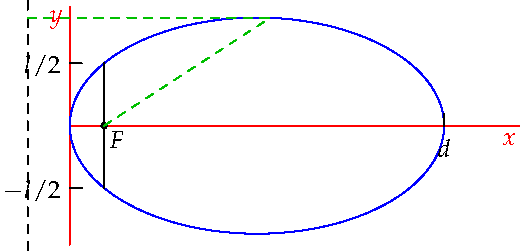
\includegraphics[width=\textwidth]{notes-01-conicellipse}\\
% $y^2=lx-\frac{lx^2}d$\\
% $\frac{(x-\frac d2)^2}{d^2/4}+\frac{y^2}{dl/4}=1$
% \end{minipage}
% \begin{minipage}{0.25\textwidth}\centering
% 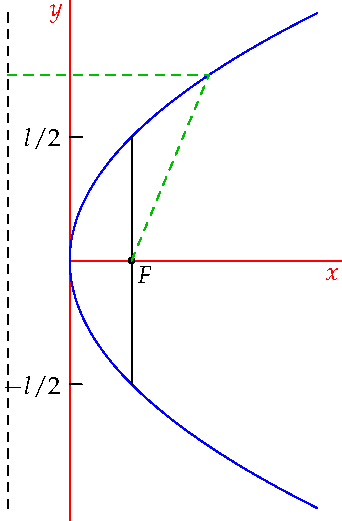
\includegraphics[width=\textwidth]{notes-02-conicparabola}\\
% $y^2=lx$
% \phantom{bob}
% \end{minipage}
% \begin{minipage}{0.35\textwidth}\centering
% 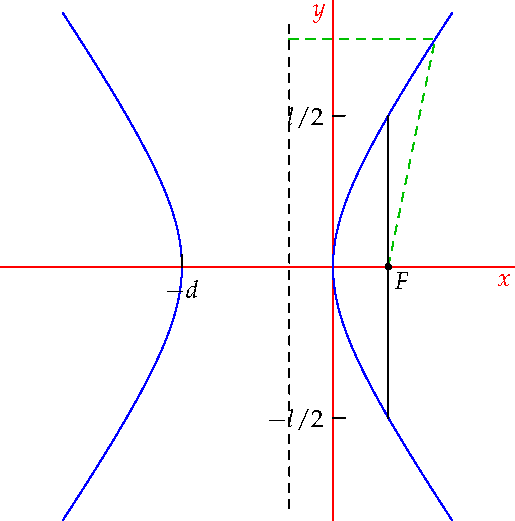
\includegraphics[width=\textwidth]{notes-03-conichyperbola}\\
% $y^2=lx+\frac{lx^2}d$\\
% $\frac{(x+\frac d2)^2}{d^2/4}-\frac{y^2}{dl/4}=1$
% \end{minipage}



 

